\documentclass[11pt]{article}

\usepackage{amsmath}
\usepackage{booktabs}
\usepackage{graphicx}
\usepackage{microtype}
\usepackage{natbib}
\usepackage{siunitx}
\usepackage{xcolor}
\usepackage{hyperref}
\usepackage{url}
\usepackage{arxivrefined}

\hypersetup{
  colorlinks=true,
  linkcolor=blue!55!black,
  citecolor=blue!55!black,
  urlcolor=blue!55!black,
  pdftitle={SIDEREA: Evidence-Bound and Human-Supervised Triage of Optical Transient Alerts},
  pdfauthor={Aadi Ajeesh Nair and Ryan Gomez},
  pdfsubject={Auditable human-supervised triage of optical transient alerts},
  pdfkeywords={time-domain astronomy, optical transients, alert brokers, human-in-the-loop systems, reproducibility}
}
\sisetup{group-separator={,},group-minimum-digits=4}
\DeclareSIUnit{\arcsec}{arcsec}
\makeatletter
\setlength{\@fptop}{0pt}
\setlength{\@fpsep}{10pt plus 1fil}
\setlength{\@fpbot}{0pt plus 1fil}
\makeatother

\newcommand{\legacycampaign}{I SPY}
\newcommand{\siderea}{SIDEREA}
\newcommand{\ztf}{ZTF}
\newcommand{\alerce}{ALeRCE}
\newcommand{\tns}{TNS}

\renewcommand{\headeright}{Nair \& Gomez}
\renewcommand{\undertitle}{Prepared for the IRIS Conference}
\renewcommand{\shorttitle}{SIDEREA: Evidence-Bound Transient Triage}

\title{\siderea: Evidence-Bound and Human-Supervised Triage of Optical Transient Alerts}

\author{
  Aadi Ajeesh Nair\\[-1pt]
  {\normalfont\small\href{mailto:aadinair310@gmail.com}{\texttt{aadinair310@gmail.com}}}
  \And
  Ryan Gomez\\[-1pt]
  {\normalfont\small\href{mailto:ryangomez.hs@gmail.com}{\texttt{ryangomez.hs@gmail.com}}}
}

\date{September 2026}

\begin{document}

\maketitle

\begin{abstract}
We present \siderea---the System for Irregular-lightcurve Discovery, Evidence-bound Ranking, and Expert Assessment---an evidence-bound pipeline for human-supervised triage of optical transient alerts. The system was developed from an audit of \legacycampaign, a small search program using public Zwicky Transient Facility alerts distributed through the ALeRCE broker. The historical pipeline ranked sources with interpretable light-curve features and then applied registry, catalog, moving-object, image, and report-wording checks. \siderea\ retains this division of labor while adding survey-aware measurements, content-addressed candidate versions, time-limited external evidence, version-bound review, and deterministic allocation of finite review capacity. Reporting is governed by a conjunction of required clearances rather than by ranking score; missing, stale, malformed, or incorrectly bound evidence cannot satisfy the gate. The campaign record contains 24 productive runs between 2026 April and July and 3,824 distinct broker objects. After removal of one duplicated pull, 223,938 of 424,223 detection rows passed the recorded quality cuts. An undocumented policy change on July 5 coincided with a decrease in the early-veto fraction from 54.5\% to 2.68\% and an increase in the shortlist fraction from 0.51\% to 13.9\%. Run-cluster bootstrap intervals for the corresponding changes are $[-0.812,-0.282]$ and $[0.098,0.171]$. These differences describe pipeline operation and do not identify a causal effect. Of 200 recorded registry checks, 30 found an existing TNS object; 55 of 193 catalog evaluations found a known or suspected variable. Two submitted objects received TNS designations, including ZTF26abdqbqw = AT~2026rsp. The current implementation passed 405 tests on Python 3.11, strict static typing, and deterministic local replay. The available record supports claims about workflow behavior and tested software invariants, but not completeness, purity, or comparative classifier performance.
\end{abstract}

\keywords{time-domain astronomy \and optical transients \and astronomical data pipelines \and alert brokers \and human-in-the-loop systems \and reproducibility}

\section{Introduction}
\label{sec:introduction}

Wide-field time-domain surveys produce alert streams that cannot be inspected exhaustively. ZTF has a $47~\mathrm{deg}^{2}$ field of view and has demonstrated nightly distributions of up to 1.2 million alerts, corresponding to roughly 70~GB \citep{bellm2019,graham2019,masci2019,patterson2019}. Its alerts are thresholded difference-image detections. The stream therefore contains transients together with variable stars, active galactic nuclei (AGN), moving objects, and subtraction residuals.

Alert brokers organize these detections into objects and provide catalog annotations, derived features, and machine-learning classifications. ALeRCE includes both stamp- and light-curve-based classifiers \citep{forster2021,carrascodavis2021,sanchezsaez2021}. Their scores are useful for prioritization, but they do not determine whether an object is previously known, whether an external query completed successfully, whether the image residual is persistent, or whether a physical classification is justified. These questions depend on different observations and have different failure modes (Figure~\ref{fig:claim-boundary}).

\begin{figure}[ht]
\centering
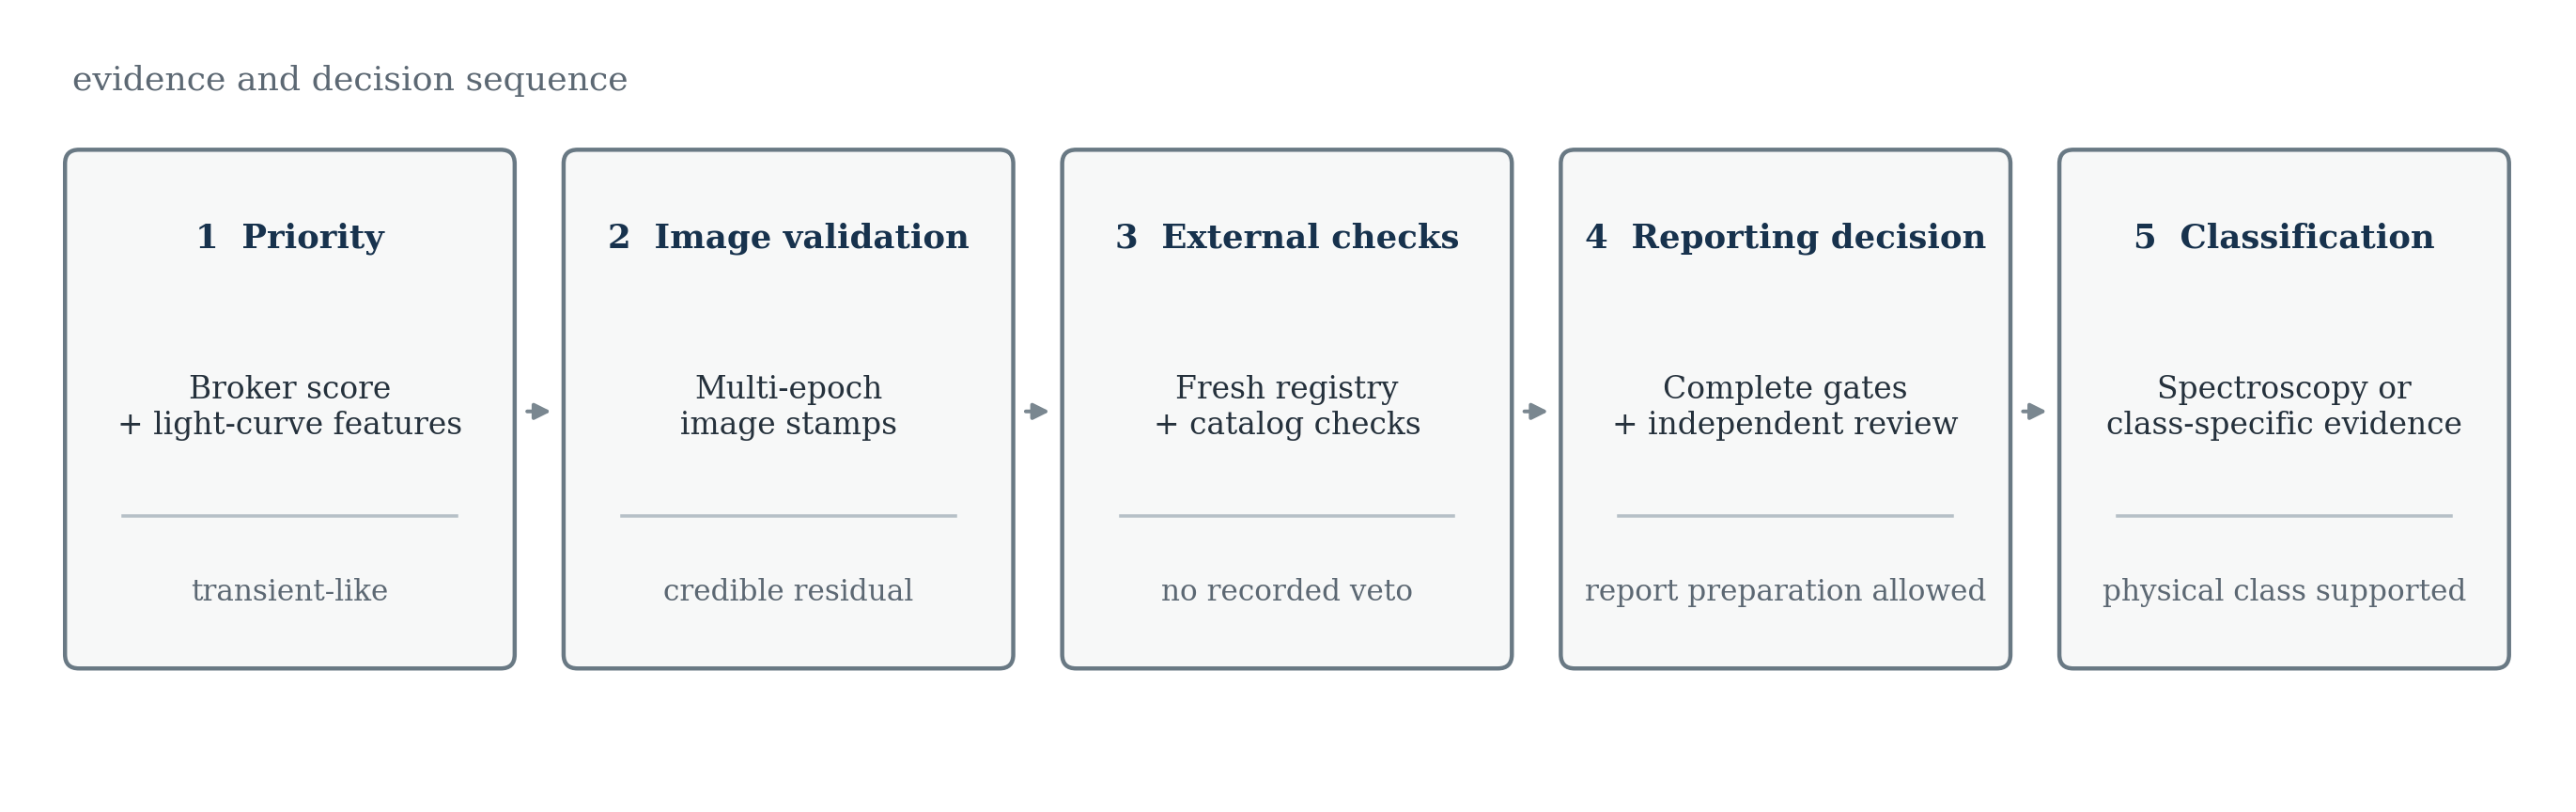
\includegraphics[width=\linewidth]{figures/claim_boundary.png}
\caption{Evidence used at successive stages of transient triage. Broker and light-curve quantities determine priority; image data address source reality; timestamped registry and catalog queries address novelty and known-source associations; the reporting decision additionally requires policy and review clearances. Physical classification generally requires information beyond the discovery photometry.}
\label{fig:claim-boundary}
\end{figure}

\legacycampaign\ was an operational filter above the public ZTF/ALeRCE stream. It combined a hand-set priority score with catalog and registry queries, light-curve and image inspection, and manual preparation of TNS reports. The campaign record is incomplete at the object level, but it preserves enough run-level information to reconstruct workload and rejection summaries. An audit of that record motivated \siderea, which stores the state of each check and binds evidence and approvals to an immutable candidate version. Neither system performs unattended submission.

This paper reports the historical campaign and describes the current implementation. Section~\ref{sec:related} places the work relative to alert brokers and follow-up systems. Sections~\ref{sec:data}--\ref{sec:methods} define the input data, score, decision states, and human review procedure. Section~\ref{sec:siderea} describes the current data and evidence model. Sections~\ref{sec:campaign}--\ref{sec:software-verification} report the campaign audit and local software verification. The available data do not support a completeness measurement, a false-negative rate, or a comparison with learned ranking methods; Section~\ref{sec:validation} specifies the prospective data needed for those analyses.

\section{Related Work}
\label{sec:related}

The modern alert ecosystem can be separated into four layers. The \emph{survey layer} performs calibrated imaging, differencing, source extraction, reliability estimation, historical association, and alert packaging \citep{masci2019,patterson2019,duev2019}. The \emph{broker layer} ingests a high-volume stream and adds searchable history, crossmatches, features, classifications, and user-defined filters. The \emph{target-and-observation layer} coordinates follow-up resources and the evolving data acquired for promising targets \citep{street2018}. Finally, a \emph{registry layer}, such as TNS, records discovery and classification reports. \legacycampaign\ is a small decision layer between broker and registry.

This position is related to, but narrower than, several established broker frameworks. AMPEL combines stream selection with user-contributed analysis, provenance, replay, and explicit ``information states'' that evolve as data accumulate; it evaluated more than 200 transient selection functions by replaying the first four months of public ZTF alerts \citep{nordin2019}. ANTARES emphasizes catalog annotation, configurable filters, provenance, and scalable event-broker architecture \citep{matheson2021}. Fink combines ingestion, annotation, filtering, redistribution, and continuously developed science modules \citep{moller2021}; an active-learning module demonstrated how purity and efficiency can be estimated when an external truth set exists \citep{leoni2022}. Lasair aggregates alerts into objects and exposes light curves, catalog crossmatches, SQL queries, and user filters \citep{smith2019}. These systems are designed for stream-scale community use; \legacycampaign\ instead tests a compact rejection protocol operated by a small reporting group.

Human review is not anomalous in this ecosystem. ALeRCE's SN Hunter presents classifier-selected objects to experts for TNS decisions \citep{carrascodavis2021}. The ZTF Bright Transient Survey (BTS) used a deliberately simple initial filter to reduce false negatives, followed by human scanning and later checks for point-source coincidence, long-term history, variables, and AGN \citep{fremling2020}. BTS subsequently constructed a magnitude-limited statistical sample and measured spectroscopic completeness as a function of limiting magnitude \citep{perley2020}. That last step is an important contrast: a reproducible filter plus human review can produce candidates, but population-level claims require a controlled parent sample, outcome labels, and a measured selection function.

Recent work has moved beyond single supervised class scores toward complementary representations and explicit top-$K$ review. Anomaly Hunter for Alerts combines separate feature, image-cutout, and light-curve autoencoders and evaluates candidates at a fixed review rank; the limited overlap among its anomaly routes shows that distinct modalities expose different failure modes \citep{iskandarli2026}. Astra-CLR learns multi-filter ZTF representations through asymmetric temporal views \citep{majumder2026}, while AstroCo targets irregular stellar light curves with a self-supervised Conformer encoder \citep{tan2025}. In the StarEmbed benchmark, general-purpose time-series representations were useful for clustering and out-of-distribution detection without uniformly surpassing established classification baselines \citep{li2026}. These results motivate a separate anomaly reserve in a review queue, but they do not justify allowing an embedding or reconstruction loss to certify novelty.

\siderea\ operates downstream of the broker rather than replacing broker functionality. Its main distinction is the representation of registry freshness, service failure, catalog associations, image review, and permitted report wording within a versioned candidate record. Learned representations are restricted to queue ordering and are not included in the reportability predicate. This division is consistent with the need for greater automation in Rubin-era transient astronomy while retaining separate controls on review and registry action \citep{rehemtulla2025}. The campaign results describe the operation of the legacy filter, and the software audit tests the reconstructed decision rules; neither is a throughput or classification benchmark against the broker systems above.

\section{Data Sources}
\label{sec:data}

\subsection{Units of analysis}

The words \emph{alert}, \emph{detection}, \emph{object}, and \emph{candidate} are often used loosely, but they are not interchangeable in this work. Table~\ref{tab:units} defines the accounting units used throughout the paper. This distinction is essential because summing detection rows measures computational workload, while counting distinct object identifiers measures sky sources, and counting repeated candidate evaluations measures operator workload.

\begin{table}[ht]
\centering
\caption{Accounting units used in the campaign audit.}
\label{tab:units}
\begin{tabular}{p{0.19\linewidth}p{0.70\linewidth}}
\toprule
Unit & Definition \\
\midrule
Alert/detection & A single epochal difference-image measurement associated with a ZTF object identifier. \\
Broker object & An ALeRCE object returned by a query; it may or may not yield a usable light curve. \\
Distinct object & A unique object identifier with a retrieved light curve, counted once across run directories. \\
Candidate evaluation & A row presented to a pipeline stage. The same astrophysical object can contribute more than one evaluation after reprocessing. \\
Packet & A prepared report bundle; packet creation is not submission. \\
Designation & A TNS registry outcome; designation is not a spectroscopic classification. \\
\bottomrule
\end{tabular}
\end{table}

\subsection{ZTF alerts through ALeRCE}

ZTF alert packets contain the current difference-image detection, historical photometry and upper limits, catalog context, and science, reference, and difference cutouts \citep{patterson2019}. The upstream ZTF Science Data System performs image subtraction and machine-learned reliability filtering before distribution \citep{masci2019,duev2019}. Consequently, the input to \legacycampaign\ is already selected twice: first by ZTF alert production, then by ALeRCE ingestion and classification. Any \legacycampaign\ selection function is conditional on both upstream layers.

The search begins with objects returned by the ALeRCE API. During the campaign the broker query targeted the light-curve classifier classes SNIa, SNII, SNIbc, and SLSN. The current campaign wrapper uses a minimum broker probability of 0.25, requests as many as 350 previously unseen objects, and restricts the query to objects first detected within the preceding 45 days. Earlier runs used related but not identical thresholds; the consequences of this evolution are discussed in Section~\ref{sec:limitations}.

For every returned ZTF object identifier, the pipeline requests the full ALeRCE detection history and caches the JSON response. The working photometry consists of the corrected PSF magnitude and uncertainty when available, falling back to the uncorrected values, together with MJD, filter identifier, coordinates, and catalog flags. ZTF filter identifiers are mapped to $g$, $r$, and $i$. The ALeRCE light-curve classifier itself also distinguishes corrected and difference photometry because the two representations carry different systematic behavior \citep{sanchezsaez2021}.

Non-detections are retained in the broker history and used during manual adjudication, but they do not enter the numerical score in Equations~\ref{eq:transient-score} and \ref{eq:combined-score}. This asymmetry is scientifically important. A compact sequence of detections preceded by deep non-detections is stronger evidence for a recent turn-on than the same detection sequence without constraining prior limits. Conversely, alternating marginal detections and non-detections near a common limit can mimic variability. The present score therefore ranks detected photometry; the human stage interprets censoring information that the score omits.

\subsection{External services and catalogs}

Four external resources provide independent rejection evidence:

\begin{enumerate}
  \item TNS is queried first by internal ZTF name and then, if necessary, by a \SI{3}{\arcsec} cone search. A candidate is not cleared when the query fails or authenticated access is unavailable.
  \item SkyBoT is queried at the candidate position and peak epoch using a \SI{10}{\arcsec} radius to identify known moving Solar System objects \citep{berthier2006}.
  \item SIMBAD is queried within \SI{3}{\arcsec} for known stellar, variable, and extragalactic counterparts \citep{wenger2000}.
  \item The AAVSO International Variable Star Index (VSX), accessed through VizieR, is queried within \SI{3}{\arcsec} \citep{ochsenbein2000,watson2006}.
\end{enumerate}

These catalog checks are intentionally conservative. A VSX association is treated as a rejection. A clearly variable-like SIMBAD object type is also rejected. A generic stellar association triggers manual review, while a galaxy, QSO, or AGN association triggers host/nuclear review and forces cautious classification language.

The adopted cone radii are operational thresholds, not association probabilities. A fixed-radius match ignores the positional uncertainties of both catalogs, the local surface density of possible counterparts, and physical information such as color or source class. Bayesian cross-identification offers a principled alternative by combining astrometric likelihoods with prior and non-spatial evidence \citep{budavari2008}. Until such a model is implemented, \legacycampaign\ uses fixed-radius matches only as conservative vetoes or review triggers and does not interpret separation alone as proof of physical association.

\section{Pipeline and Decision Protocol}
\label{sec:methods}

\subsection{Photometric cleaning}

Input columns are standardized to source identifier, position, MJD, magnitude, magnitude uncertainty, filter, and quality flag. Rows with non-finite time, magnitude, or uncertainty are removed. The multi-object campaign retains points satisfying
\begin{equation}
  0 < \sigma_m \leq 1.0~\mathrm{mag}
\end{equation}
and, where flags are present, a catalog flag not exceeding zero. At least three retained points are required in the candidate hunter. These loose initial cuts preserve recall; stronger rejection occurs through time-series features and later validation.

The cleaning stage does not perform forced photometry, estimate a per-epoch limiting magnitude, model correlated subtraction noise, or renormalize uncertainties. It relies on the photometry and corrections exposed by ALeRCE. This boundary matters: \legacycampaign\ is a triage layer, not an independent reduction of the ZTF images.

\subsection{Light-curve features}

For each source, the code pools the retained $g$, $r$, and $i$ detections and estimates a sigma-clipped median magnitude $m_{\rm med}$ and scatter $\sigma_{\rm base}$, using 3$\sigma$ clipping for up to five iterations. Because smaller magnitudes are brighter, the amplitude relative to baseline is
\begin{equation}
  A = m_{\rm med} - m_{\rm peak},
\end{equation}
where $m_{\rm peak}$ is the brightest retained measurement. A peak signal statistic is defined as
\begin{equation}
  S_{\rm peak} = \frac{A}{\sqrt{\sigma_{\rm base}^{2} + \sigma_{m,\rm peak}^{2}}}.
\end{equation}
The pipeline also counts points brighter than
\begin{equation}
  m_{\rm med} - k\sigma_{\rm base},
\end{equation}
with $k=1.5$ in the campaign hunter. A source passes the local transient-feature test if it has at least three points, $A\geq0.2$ mag, $S_{\rm peak}\geq0.8$, at least one significant point, and no significant periodicity.

Pooling filters is an exact description of the campaign code, not a recommended final estimator. Intrinsic color and asynchronous filter sampling can inflate $\sigma_{\rm base}$ or create apparent amplitude. A future implementation should compute per-band robust baselines, represent colors separately, and combine evidence in flux space. This issue does not invalidate the audit of what the code did, but it prevents the score from being interpreted as a physically homogeneous variability statistic.

Periodicity is evaluated only for histories containing at least ten points and spanning at least two days. A Lomb--Scargle periodogram \citep{vanderplas2018} searches periods from 0.1 to 200 days with five samples per peak. A false-alarm probability below $10^{-3}$ marks the source as periodic and removes it from transient consideration.

The period veto is one-sided by construction: a significant period is evidence against a one-time transient, but a non-significant period is not evidence of aperiodicity. Sparse sampling, short baselines, evolving amplitudes, aliases, and pooled passbands all reduce sensitivity. The veto therefore removes detected periodicity without claiming that retained objects are non-periodic.

The local transient score is a bounded weighted sum,
\begin{equation}
\begin{split}
T ={}& 0.45\min\left(1,\frac{A}{A_{\min}}\right)
 + 0.35\min\left(1,\frac{S_{\rm peak}}{S_{\min}}\right) \\
&+ 0.20\min\left(1,\frac{N_{\rm sig}}{N_{\rm sig,min}}\right),
\end{split}
\label{eq:transient-score}
\end{equation}
with the thresholds given above. This is a transparent triage statistic, not a calibrated probability.

\subsection{Combined ranking}

The hunter combines the local score with broker probability and two time-domain preferences. For object $i$, let $f_i$ and $l_i$ be its first and last broker detection times, $n_i$ its retained point count, and $t_\star=\max_i l_i$ the newest last-detection time in the current batch. Define the clipping operator $[x]_0^1=\min(1,\max(0,x))$. The recency, freshness, and history terms are
\begin{align}
R_i &= \left[1-\frac{t_\star-l_i}{30~\mathrm{d}}\right]_0^1, \\
F_i &= \left[1-\frac{t_\star-f_i}{\tau_F}\right]_0^1, \\
H_i &= \left[\frac{n_i}{n_H}\right]_0^1,
\end{align}
where $\tau_F=60$~d and $n_H=60$ in the current campaign wrapper. Let $P_{{\rm broker},i}$ be the ALeRCE class probability. The combined priority score is
\begin{equation}
  Q_i = 0.45T_i + 0.25P_{{\rm broker},i} + 0.15R_i + 0.15F_i - 0.10H_i.
\label{eq:combined-score}
\end{equation}
Objects failing the local transient-feature test have $Q_i$ multiplied by 0.5. An early-veto object has $Q_i$ multiplied by an additional factor of 0.35.

Equation~\ref{eq:combined-score} is a linear utility function with hand-set coefficients. It is neither trained nor calibrated. In particular, $P_{\rm broker}$ and $T$ are not conditionally independent, $R$ and $F$ share timing information, and the history penalty introduces a preference against well-sampled long-lived objects. The score orders review effort under an operational preference for recent, compact events; it must not be described as an ``AI confidence,'' discovery probability, posterior odds, or physical-class probability. Its dependence on $t_\star$ also means that the score of an otherwise unchanged object can vary with batch composition.

In the current wrapper, the early veto is activated when any of the following holds: the broker object class is QSO or AGN; the first detection is more than 45 days old relative to the newest object in the batch; the object has more than 40 detections; or the first-to-last detection baseline exceeds 90 days. A high-priority candidate must pass the transient-feature test, avoid every early veto, have $Q\geq0.60$, be no older than 60 days under the ranking definition, and contain no more than 60 retained history points.

These thresholds encode an asymmetric loss: the project accepts that some real long-lived or nuclear transients may be deferred in order to reduce the probability of an unsupported report. The campaign did not label rejected objects completely, so the magnitude of that false-negative cost is unknown.

\subsection{Sequential decision formulation}
\label{sec:decision-theory}

The operational problem is more naturally expressed as sequential decision-making than as static classification. For object $i$ at decision time $t$, let $\mathcal{D}_{i}^{\leq t}$ denote photometry and cutouts available by $t$, $\mathcal{B}_{i}^{\leq t}$ the broker annotations available by $t$, $\mathcal{X}_{i,t}$ the timestamped external-service responses, and $\mathcal{H}_{i,t}$ the saved human assessments. The admissible information is the filtration
\begin{equation}
  \mathcal{F}_{i,t}=\sigma\!\left(\mathcal{D}_{i}^{\leq t},
  \mathcal{B}_{i}^{\leq t},\mathcal{X}_{i,t},\mathcal{H}_{i,t}\right),
\label{eq:filtration}
\end{equation}
which explicitly excludes future photometry and later catalog state. Let the latent outcome $Z_i$ range over real and novel transient, previously reported transient, variable/stellar contaminant, moving object, subtraction artifact, and unresolved. For action $a$ in the set $\mathcal{U}=\{\text{reject},\text{block},\text{review},\text{report}\}$, a generic conditional Bayes risk is
\begin{equation}
  \mathcal{R}_{i,t}(a)=
  \sum_{z}L(a,z)\,\Pr(Z_i=z\mid\mathcal{F}_{i,t})
  +\lambda_{\rm h}c_{\rm h}(a)+\lambda_{\rm d}c_{\rm d}(a,t),
\label{eq:bayes-risk}
\end{equation}
where $L$ is an asymmetric scientific loss, $c_{\rm h}$ is human review cost, and $c_{\rm d}$ penalizes delay for rapidly evolving events. Duplicate or unsupported reporting should have larger loss than an additional review, while missed-event loss remains nonzero.

The key distinction is that not every action is feasible under every information state. With $C_{ij,t}$ indicating a valid, fresh completion of required gate $j$ and $M_{ij,t}$ a positive veto match, define
\begin{equation}
  G_{i,t}=\prod_{j=1}^{J} C_{ij,t}(1-M_{ij,t}).
\label{eq:gate-product}
\end{equation}
The feasible action set is $\mathcal{U}_{i,t}=\mathcal{U}\setminus\{\text{report}\}$ when $G_{i,t}=0$ and $\mathcal{U}_{i,t}=\mathcal{U}$ when $G_{i,t}=1$. The ideal decision is therefore
\begin{equation}
  a^{\star}_{i,t}=\arg\min_{a\in\mathcal{U}_{i,t}}\mathcal{R}_{i,t}(a),
  \qquad
  \tau_i=\inf\{t:a^{\star}_{i,t}\in\{\text{reject},\text{report}\}\},
\label{eq:optimal-decision}
\end{equation}
where $\tau_i$ is a stopping time with respect to $\mathcal{F}_{i,t}$. The campaign did not estimate the posterior terms in Equation~\ref{eq:bayes-risk}; its rules and score are an auditable approximation to this constrained decision problem.

Finite reviewer capacity adds a second optimization. For eligible candidates $\mathcal{C}_t$ and nightly budget $K$, an ideal queue $S_t$ solves
\begin{equation}
  S_t^{\star}=\arg\max_{S\subseteq\mathcal{C}_t,\,|S|\leq K}
  \sum_{i\in S}\left[\Delta\mathcal{R}_{i,t}^{\rm review}
  +\gamma\,\mathcal{I}(Z_i;Y_i\mid\mathcal{F}_{i,t})\right],
\label{eq:review-budget}
\end{equation}
where $\Delta\mathcal{R}^{\rm review}$ is the expected risk reduction from review, $Y_i$ is the prospective review/follow-up evidence, and $\mathcal{I}$ is conditional mutual information. The present $Q_i$ orders candidates heuristically; it does not estimate either term in Equation~\ref{eq:review-budget}. This formulation makes the scientific target precise without retroactively promoting a hand-set score into a probabilistic model.

\subsection{Typed decision states}

The scientific safety property of the workflow is a state distinction rather than a score threshold. Table~\ref{tab:states} lists the main terminal and non-terminal states. A source advances only when each required service completed and returned a result consistent with advancement. A network error, missing credential, malformed response, or stale registry result produces \texttt{blocked/unknown}; it never produces \texttt{clear}. This is analogous to the explicit tracking of changing information states in AMPEL \citep{nordin2019}.

\begin{table}[ht]
\centering
\caption{Decision-state semantics. ``Terminal'' applies to the current evidence snapshot; a newly acquired observation or corrected catalog record can justify a new evaluation.}
\label{tab:states}
\begin{tabular}{p{0.23\linewidth}p{0.15\linewidth}p{0.52\linewidth}}
\toprule
State & Status & Meaning \\
\midrule
\texttt{rejected} & Terminal & Positive evidence for a disqualifying known object, variable, moving body, artifact, or configured history/class veto. \\
\texttt{blocked/unknown} & Non-terminal & A required query failed, was skipped, or is stale; no novelty claim is permitted. \\
\texttt{needs review} & Non-terminal & Catalog or host context is ambiguous and requires a written human adjudication. \\
\texttt{reportable} & Non-terminal & All automated gates passed at a recorded time; image and wording review remain required. \\
\texttt{packet prepared} & Non-terminal & Submission materials exist; this is not evidence that TNS received them. \\
\texttt{submitted} & Non-terminal & TNS received a report; designation and attribution must still be confirmed. \\
\texttt{designated} & Registry outcome & TNS assigned an astronomical-transient name; no physical class is implied. \\
\bottomrule
\end{tabular}
\end{table}

\subsection{Failure model and decision invariants}

The main operational failure mode is a \emph{false clear}: advancing a candidate because evidence is absent when, in fact, a required observation was never obtained. The pipeline therefore separates the value returned by a service from the validity of the service call. For required gate $j$, let $C_j\in\{0,1\}$ denote successful completion and $M_j\in\{0,1\}$ denote a disqualifying match. Advancement through the automated verification layer requires
\begin{equation}
  \mathcal{A}=\bigwedge_{j=1}^{J}(C_j=1\ \land\ M_j=0).
\label{eq:advance}
\end{equation}
Thus $C_j=0$ is not logically interchangeable with $M_j=0$. A cached result additionally requires a recorded query timestamp and a freshness rule appropriate to the resource. Because TNS is a rapidly changing registry, its negative result is refreshed immediately before submission; a stable stellar-catalog result can be reused only when its provenance remains available.

This rule controls duplicate-reporting risk but cannot guarantee astrophysical validity. A successfully completed query can still return an incomplete catalog, an erroneous association, or a stale mirror. Likewise, two convincing difference-image residuals can share a persistent subtraction defect. The workflow therefore uses defense in depth: service completion, catalog content, image morphology, temporal behavior, and claim wording address different failure modes and do not substitute for one another.

Four invariants define the intended implementation: (1) every advance has a successful, timestamped result for each required gate; (2) every rejection records the positive evidence and rule version that caused it; (3) packet preparation, submission, designation, and physical classification remain separate states; and (4) no physical label in a report is stronger than the recorded evidence. These invariants are testable properties of the decision log, unlike an informal assertion that the pipeline is ``conservative.''

\subsection{Automated verification}

Shortlisted candidates pass through two independent modules. The first checks SkyBoT, refreshes ALeRCE light-curve and stamp labels, and queries TNS. A positive SkyBoT or TNS match is a rejection. A failed or skipped TNS query is a blocking state, not a negative result.

The second module queries SIMBAD and VSX. Any VSX result within the search radius is rejected. SIMBAD object-type strings are mapped to four outcomes: variable-like matches are rejected; stellar matches require review; extragalactic matches require host/nuclear review; and other catalog matches require review. Only a source with no VSX or SIMBAD association passes automatically.

The match policy maximizes caution rather than classification accuracy. In a crowded field, a catalog source can lie within \SI{3}{\arcsec} by chance; in a sparse field, a real counterpart can lie outside the radius because of astrometric error or proper motion. Consequently, the code's catalog decision is an operational flag. It is not a posterior association probability, and a catalog non-match is not proof that no counterpart exists.

The final automated gate again rejects ALeRCE transient labels QSO or AGN, stamp labels VS, AGN, or BOGUS, candidate ages above 60 days, more than 50 detections, or baselines above 120 days. These final thresholds are partly redundant with intake thresholds by design: they prevent a candidate from becoming reportable merely because it entered through an older run configuration.

\subsection{Manual inspection and reporting}

Automation ends before submission. A human screener inspects the ALeRCE object page in a fixed order: metadata, difference-magnitude light curve, finding chart, science/template/difference stamps on every available detection date, classifier panels, magnitude statistics, and crossmatches. At least two dates must show a compact positive residual at a consistent position. Single-frame residuals, positive--negative dipoles, saturated-star halos, subtraction edges, ghosts, and unstable residual morphology are rejection reasons. These are known classes of difference-image failure; upstream real--bogus models address related radiation-hit, optical-ghost, registration, and noise artifacts statistically \citep{duev2019}, while the \legacycampaign\ review asks whether the residual remains credible across the complete available epoch sequence.

The wording gate distinguishes an unclassified optical transient from a possible nuclear/AGN-like event. A counterpart within approximately \SI{1}{\arcsec}, together with elevated AGN probability or a nuclear position, prevents supernova wording. A report packet contains the draft report, machine-readable TNS JSON, recent photometry, and the verification summaries. The current protocol requires a reviewer distinct from the screener before submission and a final TNS recheck immediately before sending. The historical campaign did not record two independent stamp labels, so inter-reviewer agreement cannot be estimated retrospectively.

Figure~\ref{fig:workflow} shows the advancement path and its three distinct terminal or blocking outcomes.

\begin{figure}[ht]
\centering
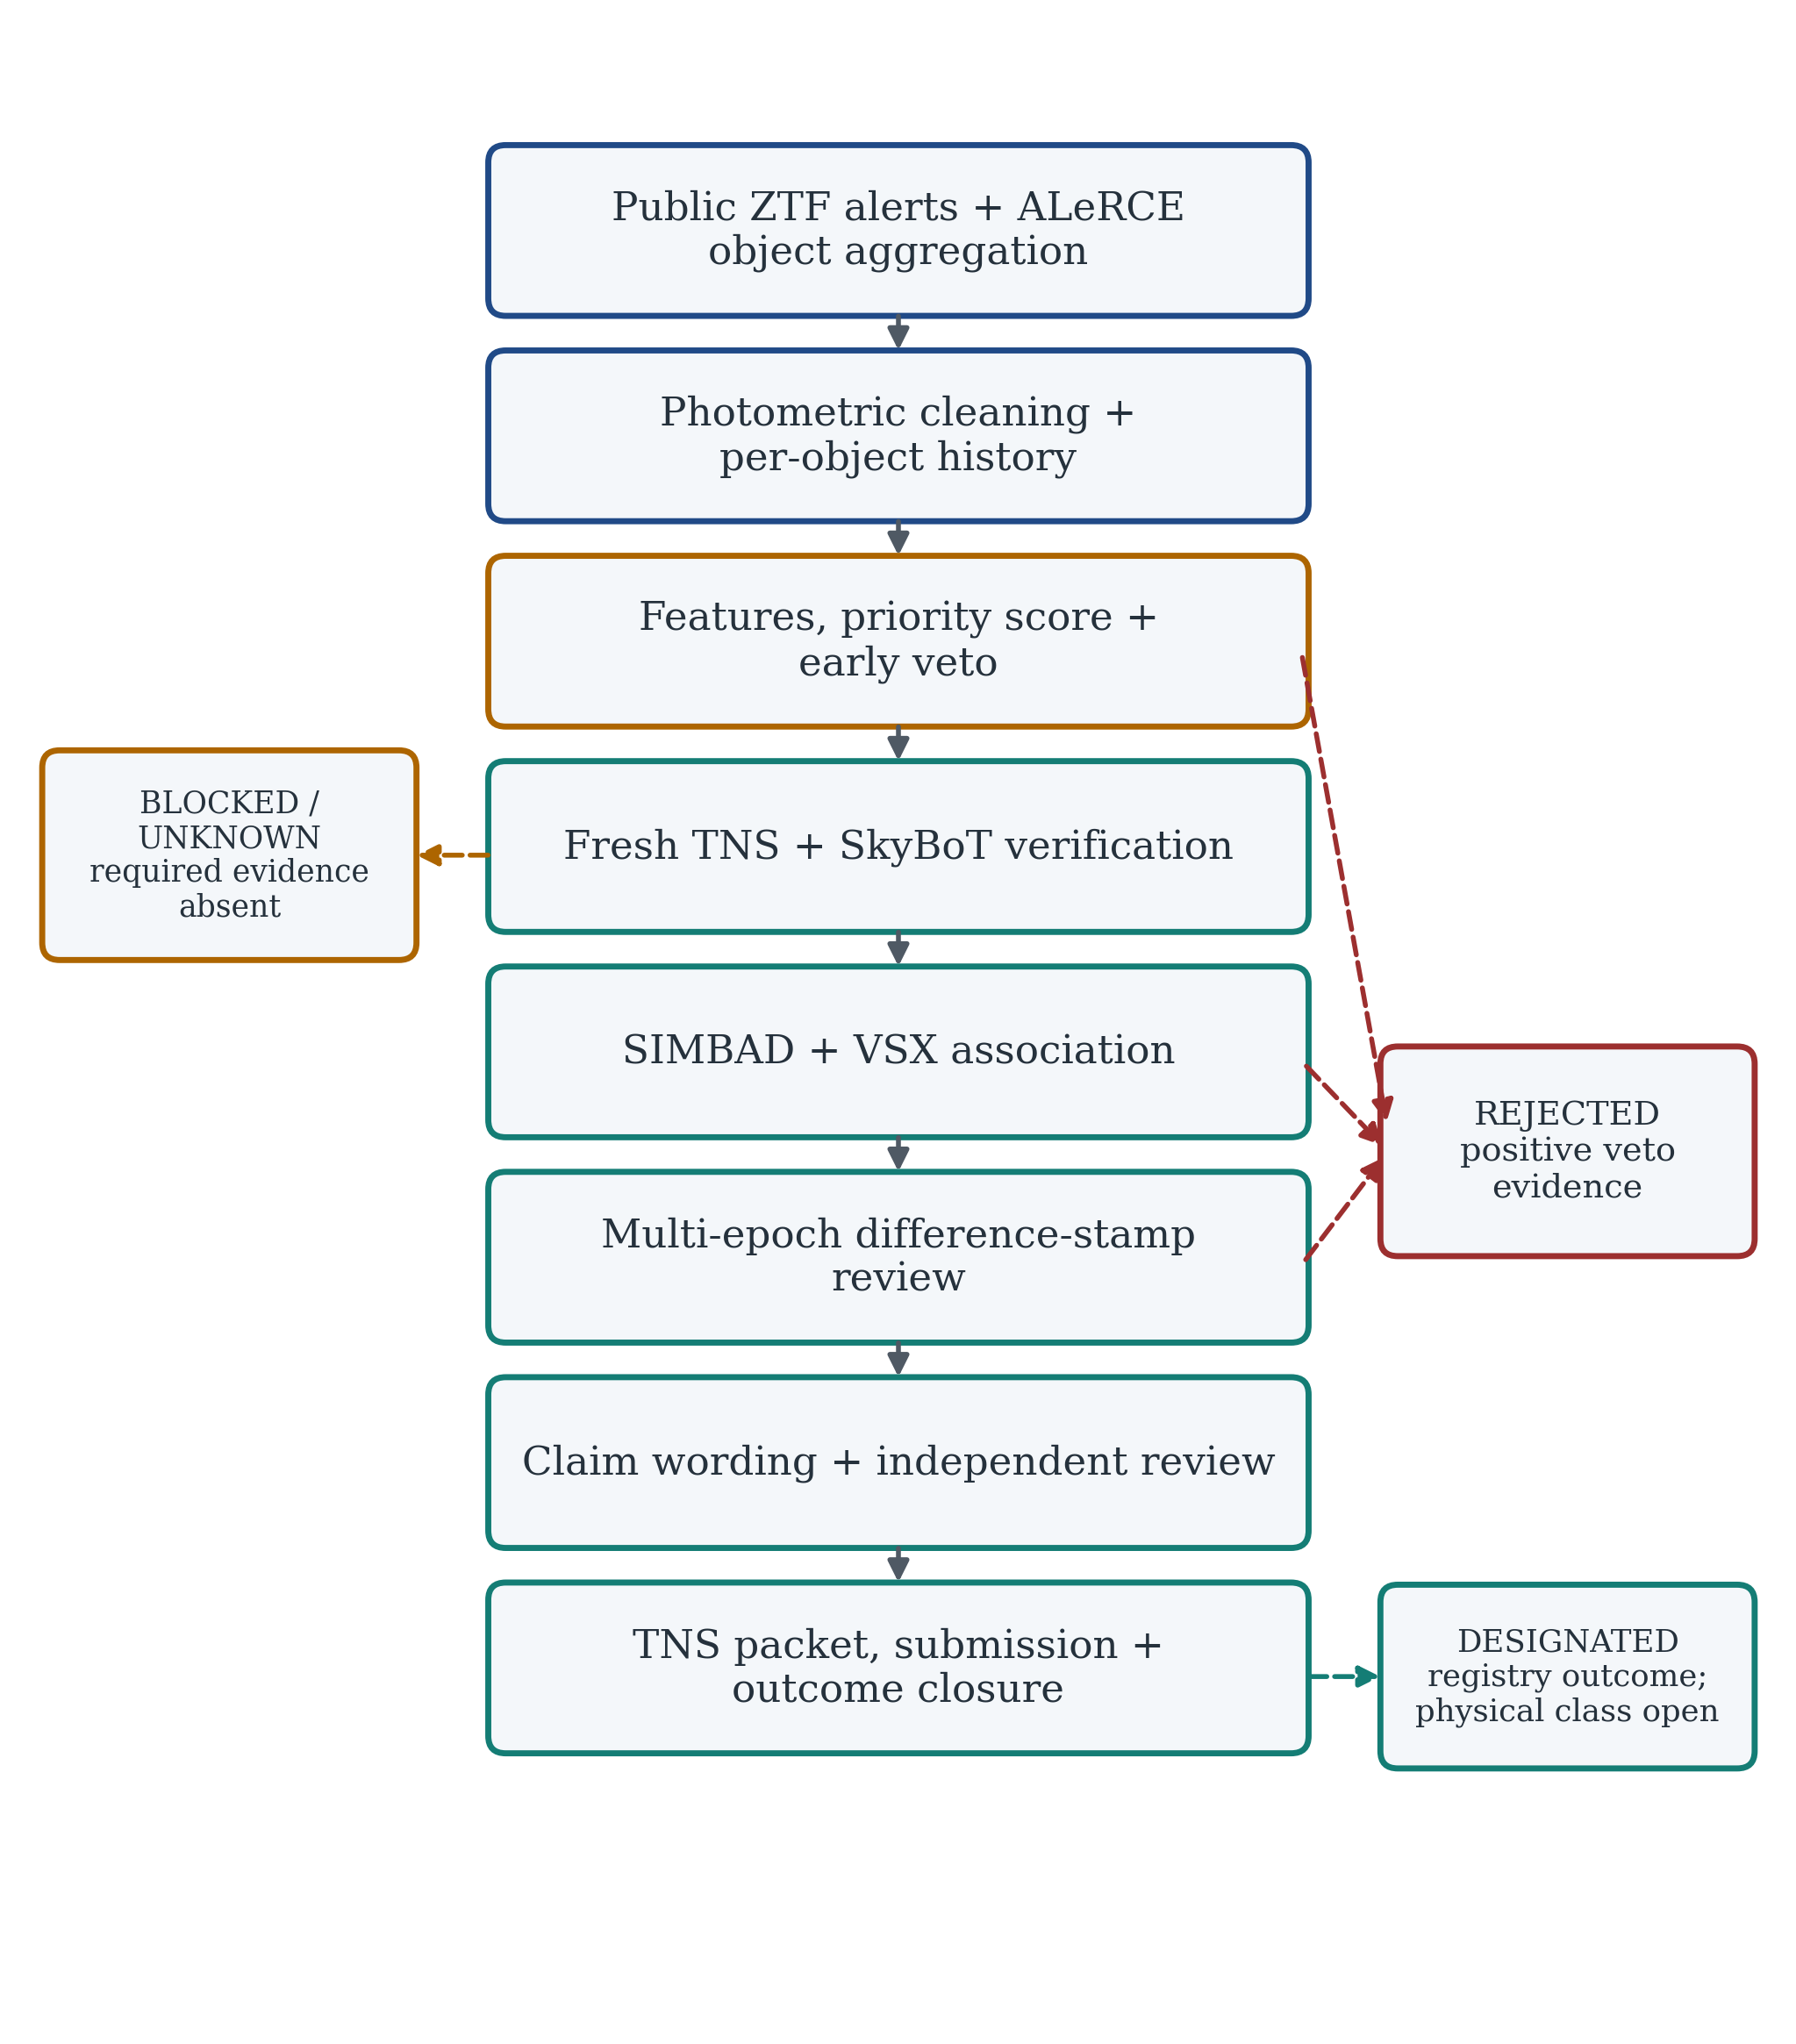
\includegraphics[width=\linewidth]{figures/pipeline_flow.png}
\caption{Legacy \legacycampaign\ workflow. Solid arrows show candidate advancement; dashed arrows show rejection, blocking, and registry outcomes. A negative query result is accepted only when the query completed successfully, so an unavailable required service cannot produce a false clearance.}
\label{fig:workflow}
\end{figure}

\section{SIDEREA Implementation}
\label{sec:siderea}

The campaign used procedural controls that were not represented consistently in its saved run artifacts. In \siderea, provenance, external checks, and review decisions are stored as typed records. Figure~\ref{fig:siderea-architecture} summarizes the implementation. Measurements and configuration determine candidate identity; external-service results are validated and bound to that identity; and review and reporting operate on the resulting versioned dossier. The system accepts either a bounded broker snapshot or a local measurement table and does not include unattended registry submission.

\begin{figure}[!htbp]
\centering
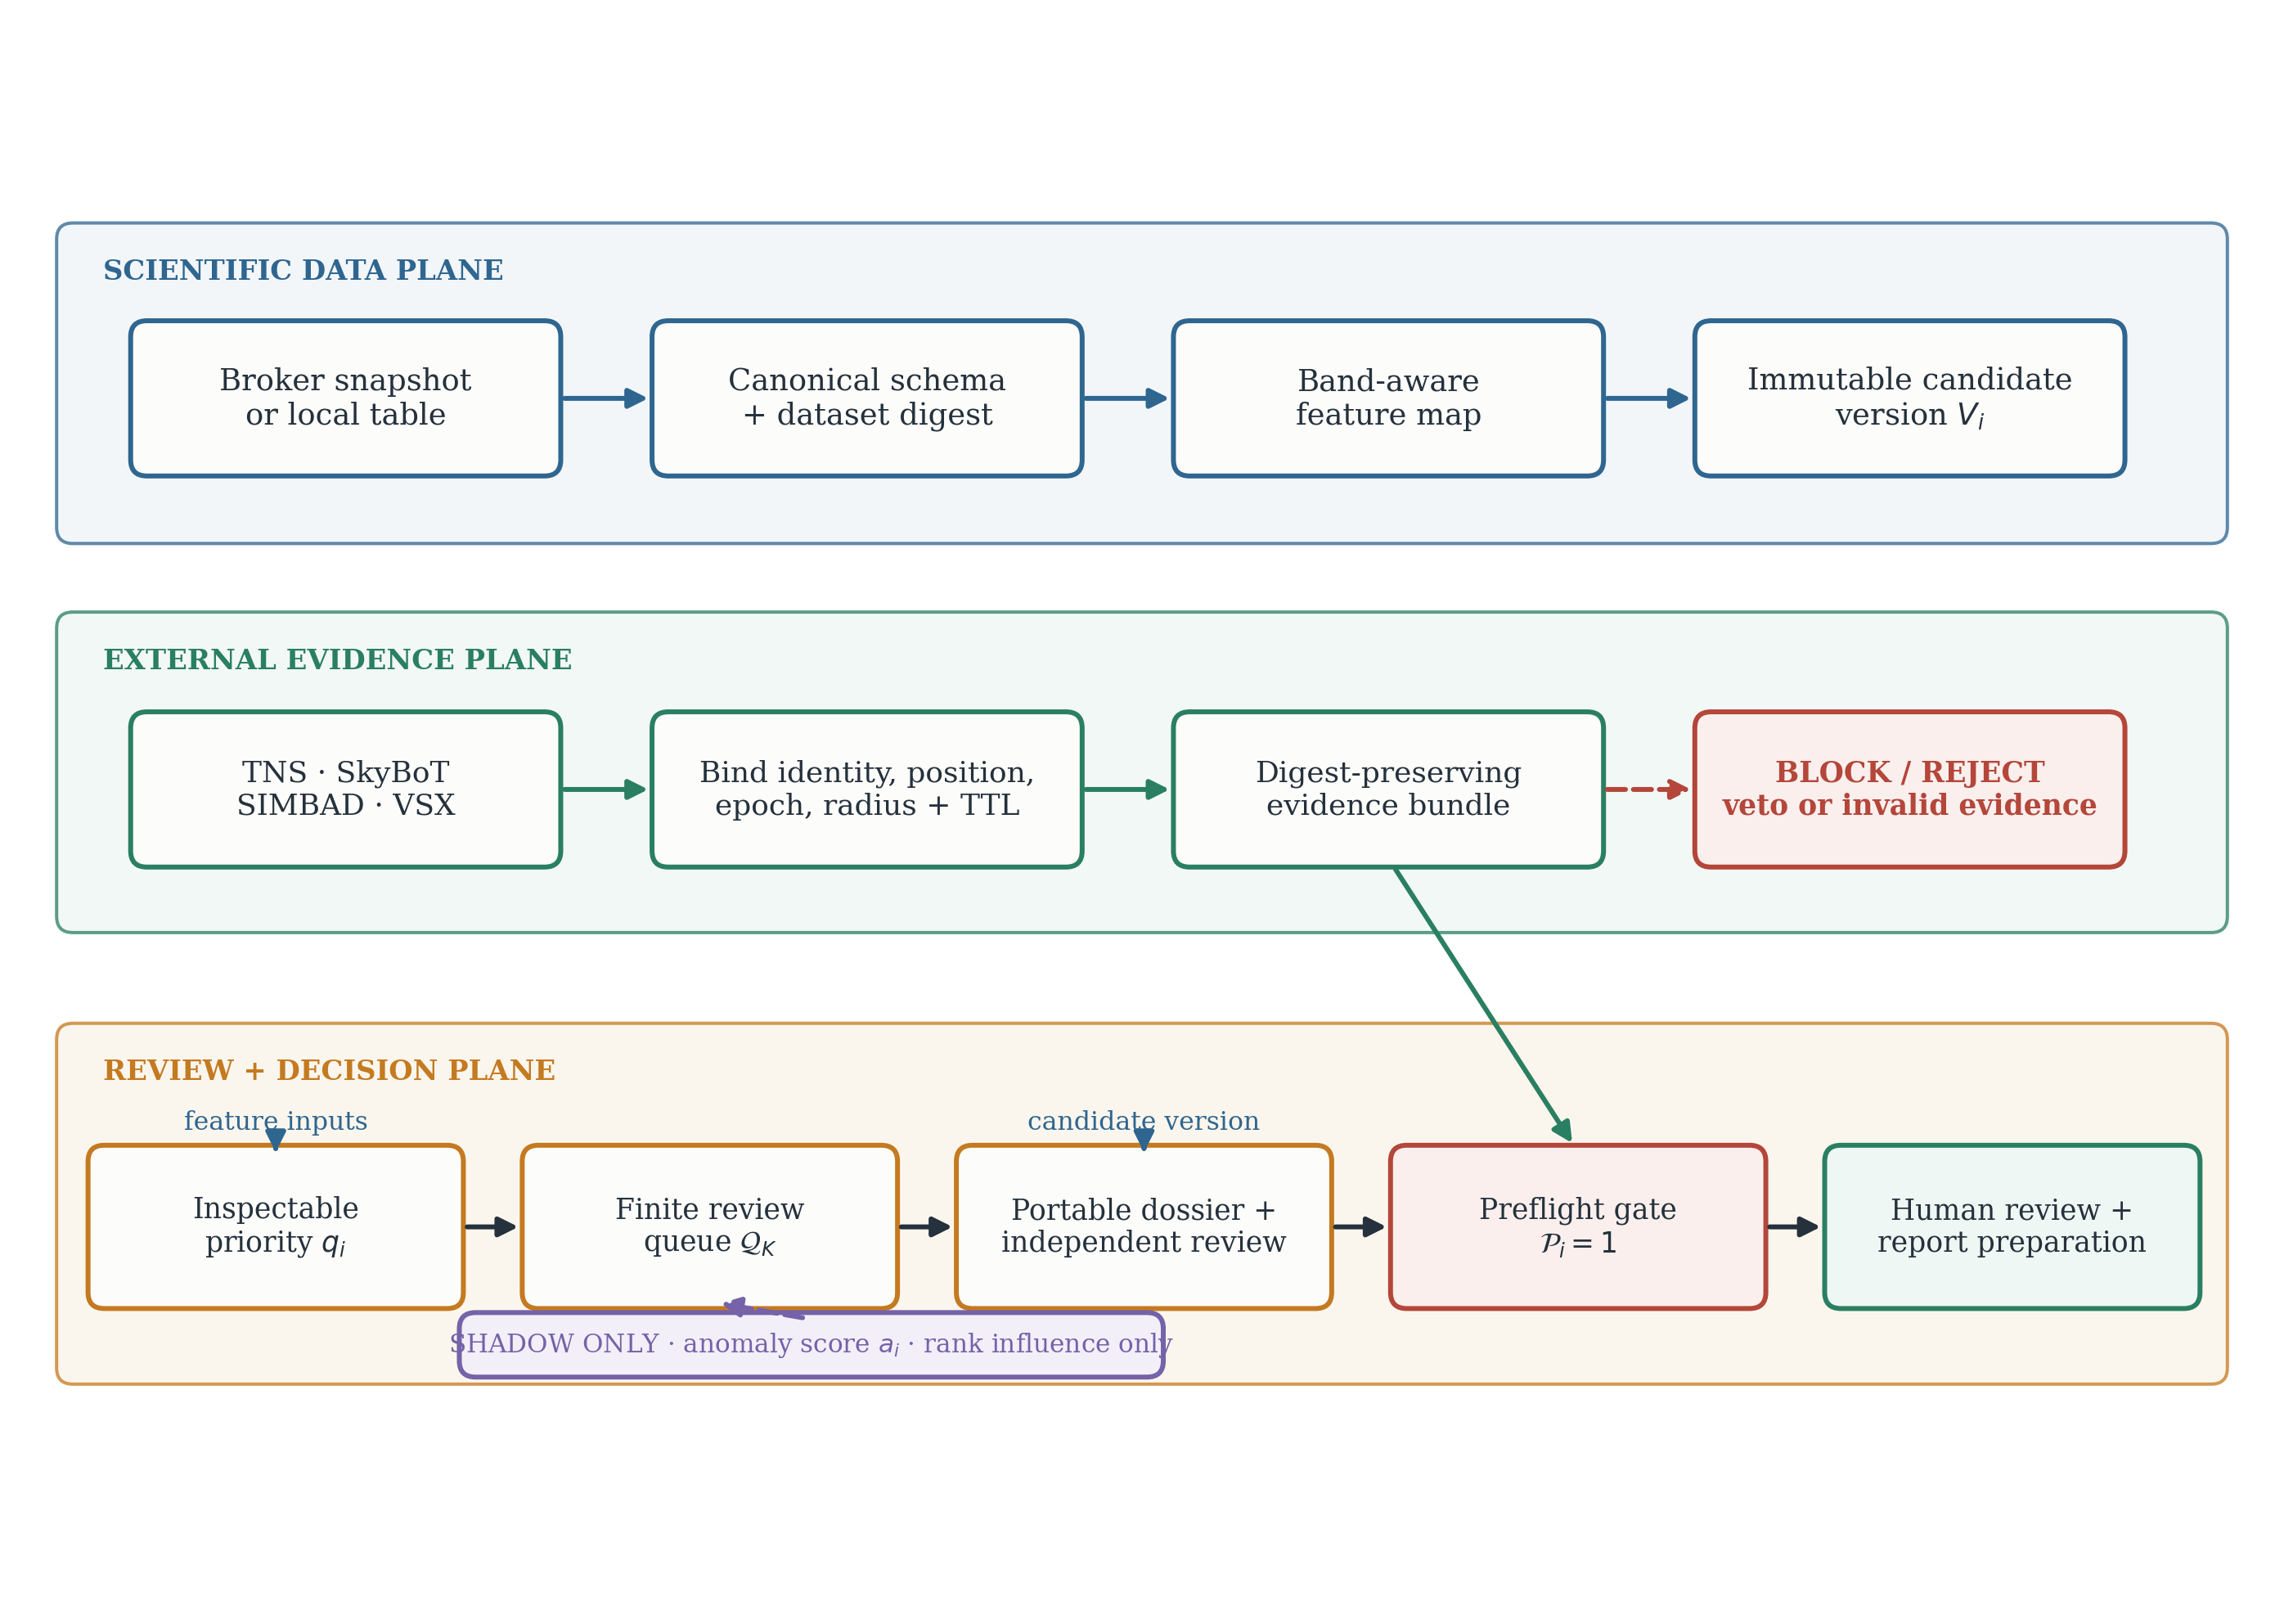
\includegraphics[width=\linewidth]{figures/siderea_architecture.png}
\caption{Implemented \siderea\ architecture as three coupled planes. Solid arrows carry authoritative state. External results are useful only after their identity, position, radius, epoch, lifetime, and response digest are bound to the candidate version. The violet shadow route may change review order but has no path around the red preflight gate.}
\label{fig:siderea-architecture}
\end{figure}

\subsection{Canonical observations and band-aware features}

An input measurement is represented as
\begin{equation}
  o_{ij}=\left(t_{ij},b_{ij},y_{ij},\sigma_{ij},d_{ij},q_{ij},u_{ij}\right),
\label{eq:observation-tuple}
\end{equation}
where $t$ is time, $b$ passband, $y$ a magnitude or supplied flux, $\sigma$ its uncertainty, $d$ an explicit detection indicator, $q$ quality state, and $u$ the measurement-unit or representation metadata. Detection status is never inferred from the sign of a difference flux. Missing uncertainty remains missing, negative difference flux remains signed, and limiting magnitudes remain non-detections. Alias ambiguity, inconsistent coordinates, and duplicate observation identities are rejected before features are evaluated.

For each passband $b$, the versioned feature map $\phi_b(\{o_{ij}:b_{ij}=b\})$ computes robust amplitude, peak contrast, uncertainty-aware significance, temporal slopes, sampling support, and prior non-detection contrasts. The aggregate map preserves the contributing band and basis. Magnitude evidence is preferred, while supplied forced/difference flux can provide an explicitly labeled fallback. This removes the historical score's pooling of asynchronous $g$, $r$, and $i$ magnitudes into a single baseline, without claiming that supplied flux has been independently calibrated or acquired by \siderea.

The current heuristic emits a bounded decomposition
\begin{equation}
  q_i=\sum_{k=1}^{6}w_k h_{ik},
  \qquad h_{ik}\in[0,1],\quad w_k\geq0,\quad \sum_k w_k=1,
\label{eq:siderea-score}
\end{equation}
over amplitude, significance, temporal shape, prior non-detection, sampling, and data-quality components. It is recorded as \texttt{is\_probability=false}. A missing measurement basis generates a warning and a conservative component value rather than an imputed astrophysical measurement.

\subsection{Content-addressed scientific identity}

Let $\mathrm{H}$ denote SHA-256 over canonical JSON. The immutable candidate version is schematically
\begin{equation}
\begin{split}
  V_i=\mathrm{H}(&\text{schema},\text{pipeline version},i,\text{campaign},
  \mathrm{H}(\mathcal{O}_i),Q_i,\phi_i,q_i,\\
  &\mathcal{E}_i,G_i,\Theta_{\rm scientific}),
\end{split}
\label{eq:candidate-version}
\end{equation}
where $\mathcal{O}_i$ is the normalized observation set, $Q_i$ the local quality decision, $\mathcal{E}_i$ external evidence, $G_i$ the gate outcome, and $\Theta_{\rm scientific}$ the relevant policy configuration. Run identifier, wall-clock execution time, and filesystem path are excluded from $V_i$ when they do not change scientific evidence. They remain in the execution manifest. A change in photometry, service evidence, gate policy, or score inputs creates a new version for which earlier human approvals do not count.

Every completed clearance is bound to candidate identifier, position, minimum search radius, configured maximum time-to-live, and---for SkyBoT---an allowed observation epoch. The raw response digest and service status are retained. A nominally clear result with an empty digest, inconsistent identity, displaced coordinates, insufficient radius, excessive lifetime, or wrong epoch is downgraded to an error before reportability is evaluated.

\subsection{Fail-closed reportability and its monotonicity}

For mandatory services $s\in\mathcal{S}$, define binary predicates $C_{is}$ (explicit clear), $B_{is}$ (correctly bound), $F_{is}$ (fresh), and $D_{is}$ (response digest present). Let $Q_i$ denote local quality clearance, $U_i$ the absence of unresolved manual ambiguity, and $A_i$ valid version-bound approvals from a screener and the required reviewers, including at least one different person. The implemented preflight predicate is
\begin{equation}
  \mathcal{P}_i
  =Q_iU_iA_i\prod_{s\in\mathcal{S}}C_{is}B_{is}F_{is}D_{is}.
\label{eq:preflight-predicate}
\end{equation}
Reporting preparation is permitted only if $\mathcal{P}_i=1$; an empty mandatory-service set is itself invalid.

\paragraph{Fail-closed monotonicity.}
Equip the evidence state with the partial order $e'\preceq e$ when $e'$ is obtained by replacing one or more valid clear predicates in $e$ by zero without changing any zero to one. Then
\begin{equation}
  e'\preceq e \quad\Longrightarrow\quad
  \mathcal{P}_i(e')\leq\mathcal{P}_i(e).
\label{eq:monotonicity}
\end{equation}
The proof is immediate because Equation~\ref{eq:preflight-predicate} is a product of binary predicates: replacing a factor of one by zero cannot increase the product. Operationally, transport failure, staleness, malformed content, incomplete binding, or approval invalidation can close a gate but cannot open it. This is a software safety property, not a claim that all catalogs are complete or correct.

\subsection{Finite review and non-authoritative representation learning}

For an eligibility set $\mathcal{E}$, review budget $K$, and anomaly reserve $m\leq K$, the deterministic allocator constructs
\begin{equation}
  \mathcal{Q}_K=operatorname{Top}_{K-m}(q_i:i\in\mathcal{E})
  \cup
  \operatorname{Top}_{m}(a_i:i\in\mathcal{E}\setminus\mathcal{Q}_{K-m}),
\label{eq:queue-allocation}
\end{equation}
with stable identifier tie-breaking. Here $a_i$ may be an anomaly score derived from engineered features or a learned embedding. The separate reserve prevents a high anomaly score from silently replacing the primary ranking and makes its review cost explicit.

The experimental irregular-time joint-embedding predictive architecture masks contiguous temporal windows and predicts their latent representations from the remaining context. Its target encoder is updated by an exponential moving average, and normalization is recomputed from unmasked context so hidden target values cannot determine the context scale. This route is shadow-only: $a_i$ can affect membership in $\mathcal{Q}_K$, but it does not occur in Equation~\ref{eq:preflight-predicate}. No result in this paper establishes that these embeddings improve astrophysical discovery.

\section{Campaign and Results}
\label{sec:campaign}

\subsection{Campaign accounting}

The operating record covers 2026 April 7 through July 30. Thirty-one run directories were recorded, of which 24 retrieved broker objects. Seven zero-object runs were attributed to DNS failures against the ALeRCE API and are excluded from scientific totals because they are failed observations of the service, not null astronomical searches. One productive run reprocessed the same 150-object pull as an immediately preceding run; unique-object totals were therefore derived from cached light-curve identifiers rather than summed query counts.

Table~\ref{tab:headline} summarizes the campaign. Approximately marked values are sums across productive runs and may include an object evaluated in more than one processing pass. The defensible object-level denominator is 3,824 distinct fetched light curves.

\begin{table}[ht]
\centering
\caption{Campaign headline statistics.}
\label{tab:headline}
\begin{tabular}{lr}
\toprule
Quantity & Value \\
\midrule
Recorded run directories & 31 \\
Productive runs & 24 \\
Non-duplicate productive pulls & 23 \\
Distinct objects with retrieved light curves & 3,824 \\
Detection rows processed & $\sim$438,600 \\
Rows surviving quality cuts & $\sim$231,700 \\
Detection rows after removing known duplicate pull & 424,223 \\
Clean rows after removing known duplicate pull & 223,938 (52.8\%) \\
Ranked candidate evaluations & $\sim$1,652 \\
High-priority shortlist evaluations & 256 \\
Fresh-shortlist evaluations & 239 \\
Individual report packets & 3 \\
Additional bulk-draft objects & 2 \\
Submitted and designated objects & 2 \\
Credited discovery with complete case record & 1 \\
\bottomrule
\end{tabular}
\end{table}

The exclusion ledger contained 6,270 broker-returned identifiers by the final run. This exceeds the number of retrieved light curves because an identifier could be marked seen even when its light curve was not successfully fetched. We consequently do not use the ledger size as the screened-object denominator.

The campaign also contains a sharp configuration/behavior discontinuity. The 2026 July 5 05:01 UTC run recorded 329 early vetoes and no high-priority objects; the 16:14 UTC run recorded 24 early vetoes and 72 high-priority objects. The following runs continued in the more permissive regime. Because no contemporaneous change log identifies the exact causal edit and intent, this discontinuity cannot be interpreted as an astrophysical change. It is evidence that configuration provenance is part of the scientific data.

\subsection{Derived operational diagnostics}
\label{sec:run-diagnostics}

We re-parsed the run table in the operating record with a reproducible figure script. For run $r$, define the five diagnostic ratios
\begin{equation}
\rho_r=\left(
\frac{C_r}{D_r},
\frac{S_r}{O_r},
\frac{R_r}{S_r},
\frac{E_r}{O_r},
\frac{L_r}{O_r}
\right),
\label{eq:run-ratios}
\end{equation}
where $O_r$, $D_r$, $C_r$, $S_r$, $R_r$, $E_r$, and $L_r$ are respectively query objects, detection rows, clean rows, sources, ranked sources, early vetoes, and shortlist entries. A ratio is missing rather than zero when its historical field was not recorded. Figure~\ref{fig:run-heatmap} displays these quantities without imputing absent cells.

\begin{figure}[p]
\centering
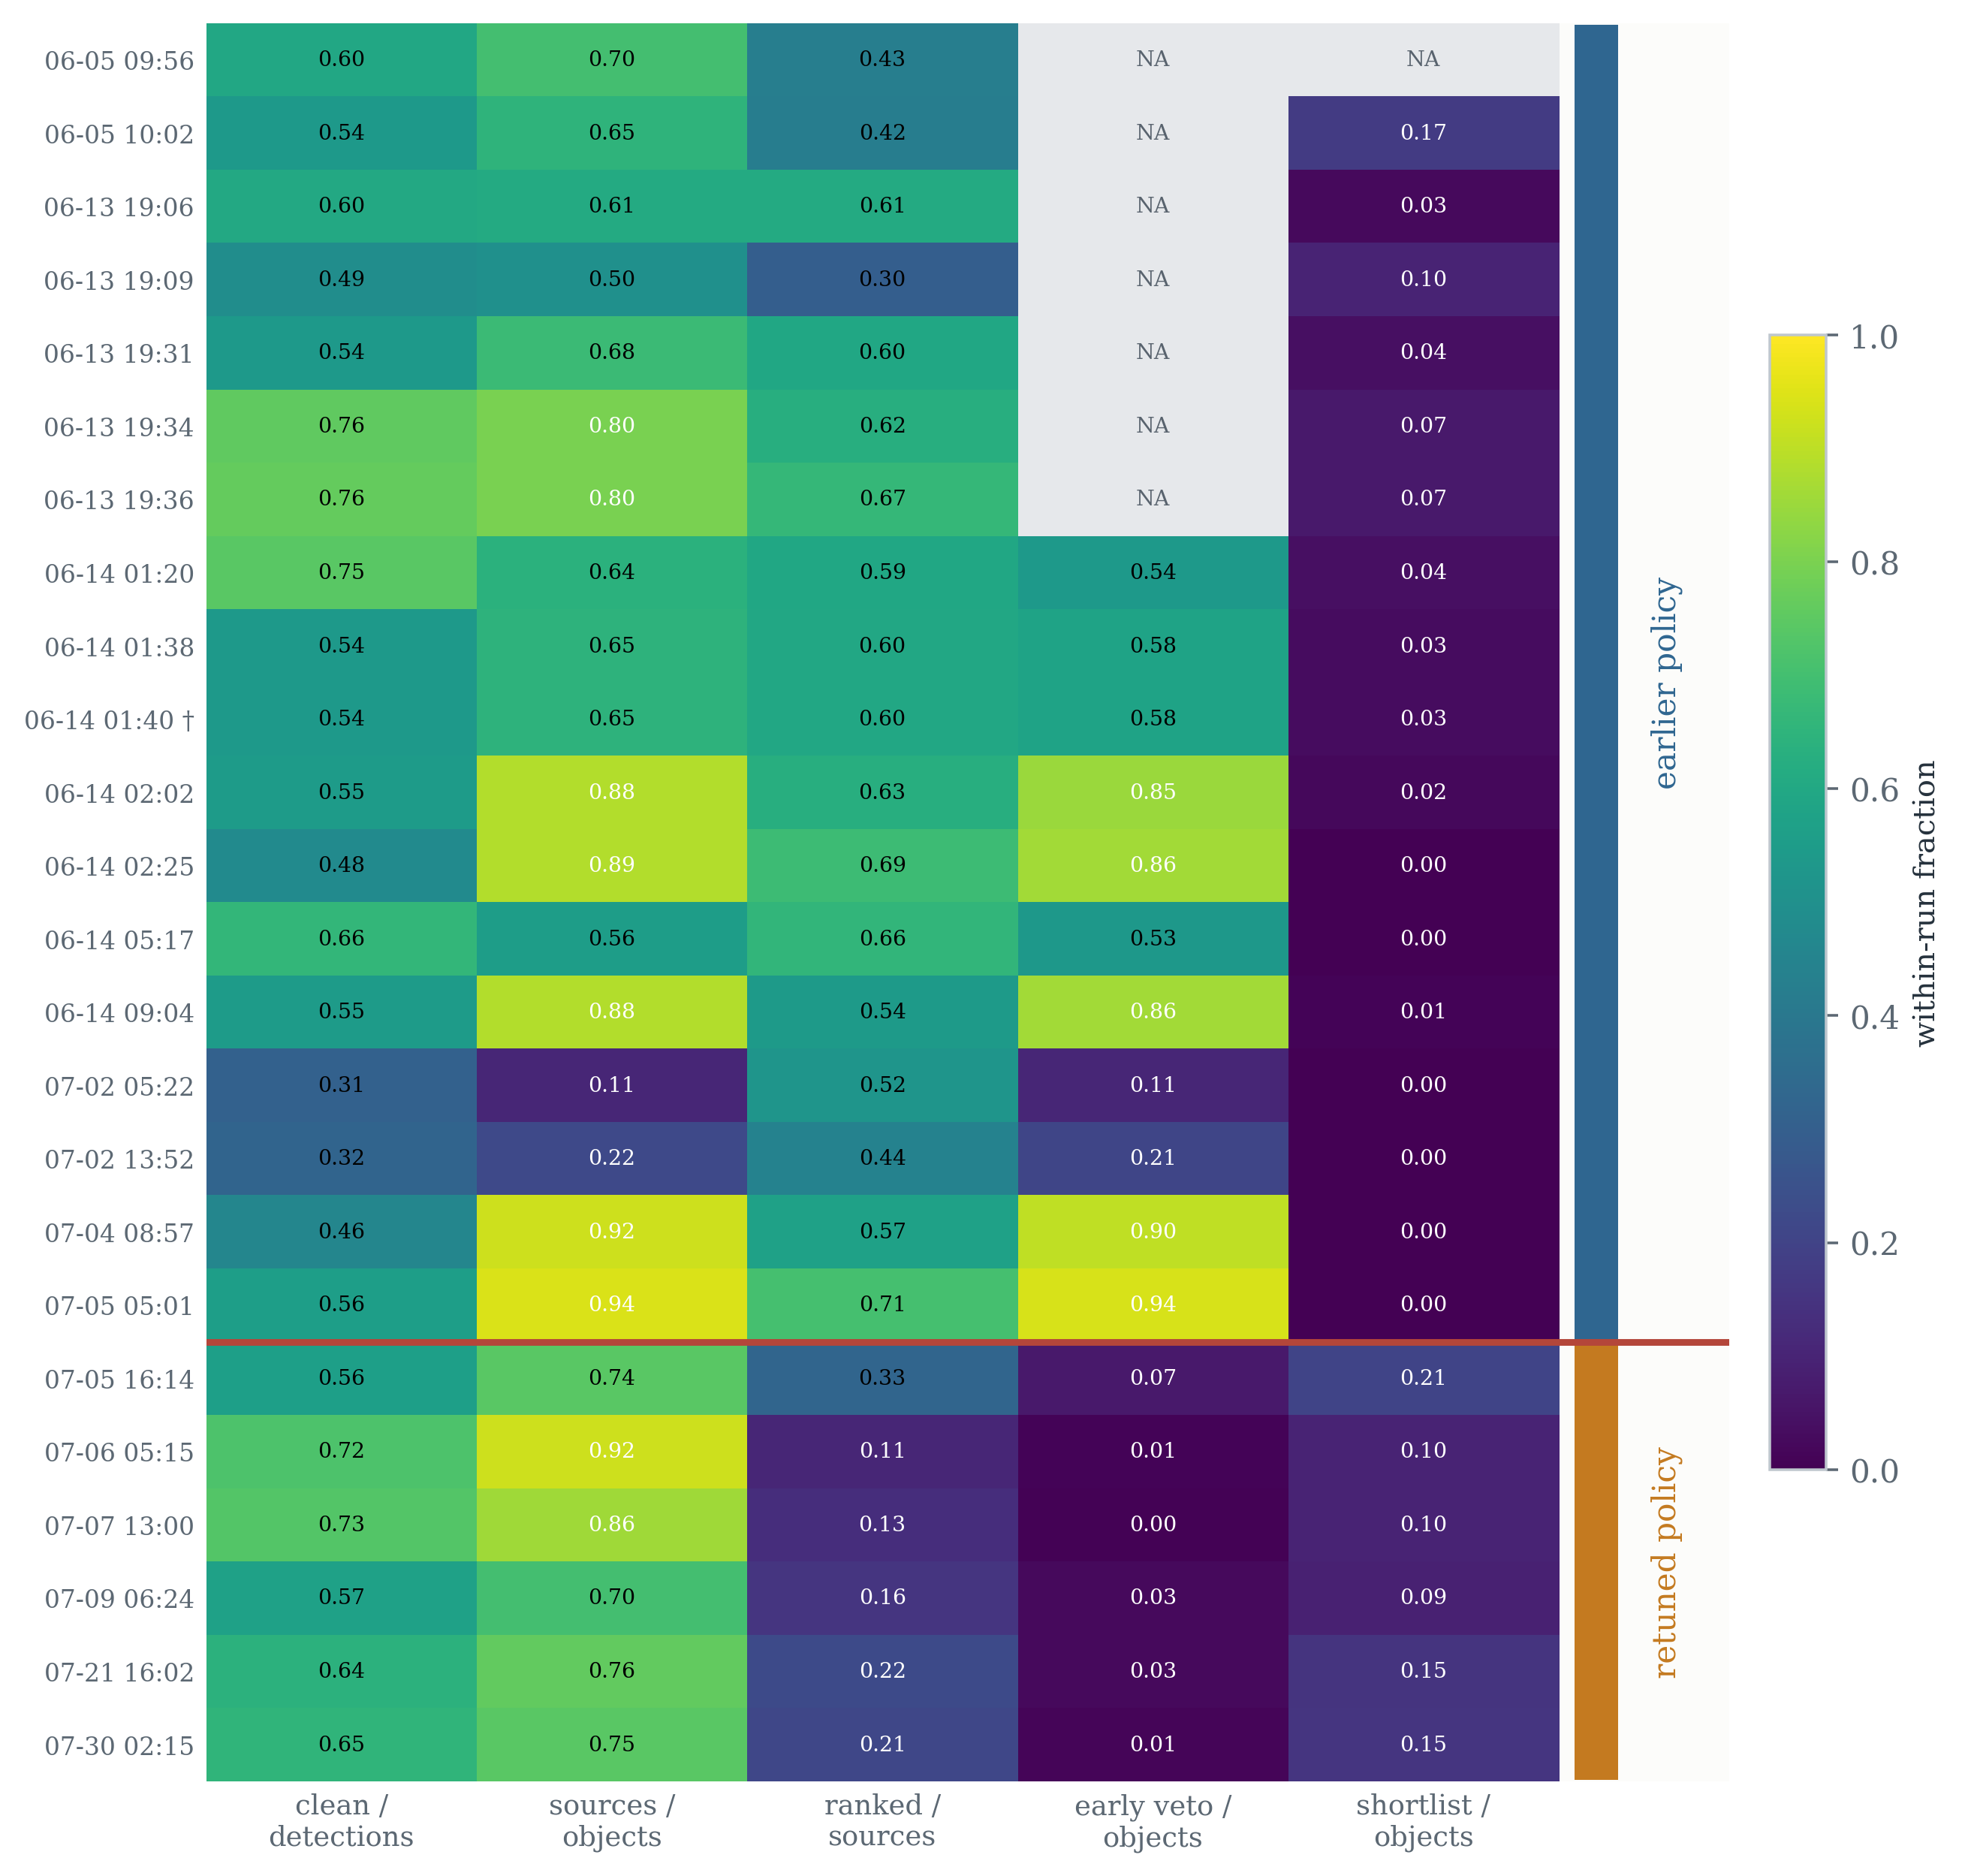
\includegraphics[width=0.88\linewidth]{figures/run_diagnostic_heatmap.png}
\caption{Heatmap of within-run diagnostic ratios for all 24 productive run records. The dagger identifies the documented duplicate pull, gray denotes unrecorded fields, and the red boundary marks the observed policy-regime discontinuity. Values describe pipeline behavior within each run; they are not detection efficiencies relative to the sky.}
\label{fig:run-heatmap}
\end{figure}

For an additive workload quantity $X_r$, the correct pooled ratio over a set of run records $\mathcal{G}$ is the ratio of sums, not the mean of run-wise ratios:
\begin{equation}
  \widehat{\rho}_{X/Y}(\mathcal{G})=
  \frac{\sum_{r\in\mathcal{G}}X_r}{\sum_{r\in\mathcal{G}}Y_r}.
\label{eq:pooled-ratio}
\end{equation}
Removing the one known duplicate pull leaves 23 run pulls containing 424,223 detection rows and 223,938 clean rows, hence $\widehat{\rho}_{C/D}=0.5279$. This 52.8\% measures row retention conditional on the recorded query and quality rule; it is not transient-detection efficiency.

For the ten non-duplicate pre-retune runs with both veto and shortlist fields, 1,922/3,525 query-object evaluations were early-vetoed (54.5\%) and 18/3,525 were shortlisted (0.51\%). For the six recorded post-retune runs, the corresponding fractions were 41/1,531 (2.68\%) and 213/1,531 (13.9\%). Thus the shortlist fraction increased by a factor of
\begin{equation}
  \frac{213/1531}{18/3525}=27.25,
\end{equation}
while the early-veto fraction decreased by a factor of $0.0491$. These contrasts quantify a policy change, not improved sensitivity: the run groups differ in date, query composition, and undocumented configuration details. Figure~\ref{fig:campaign-dynamics} shows that the discontinuity coincides with a sharp fall in recorded per-run row volume as well as a transfer of rejection burden downstream.

\begin{figure}[p]
\centering
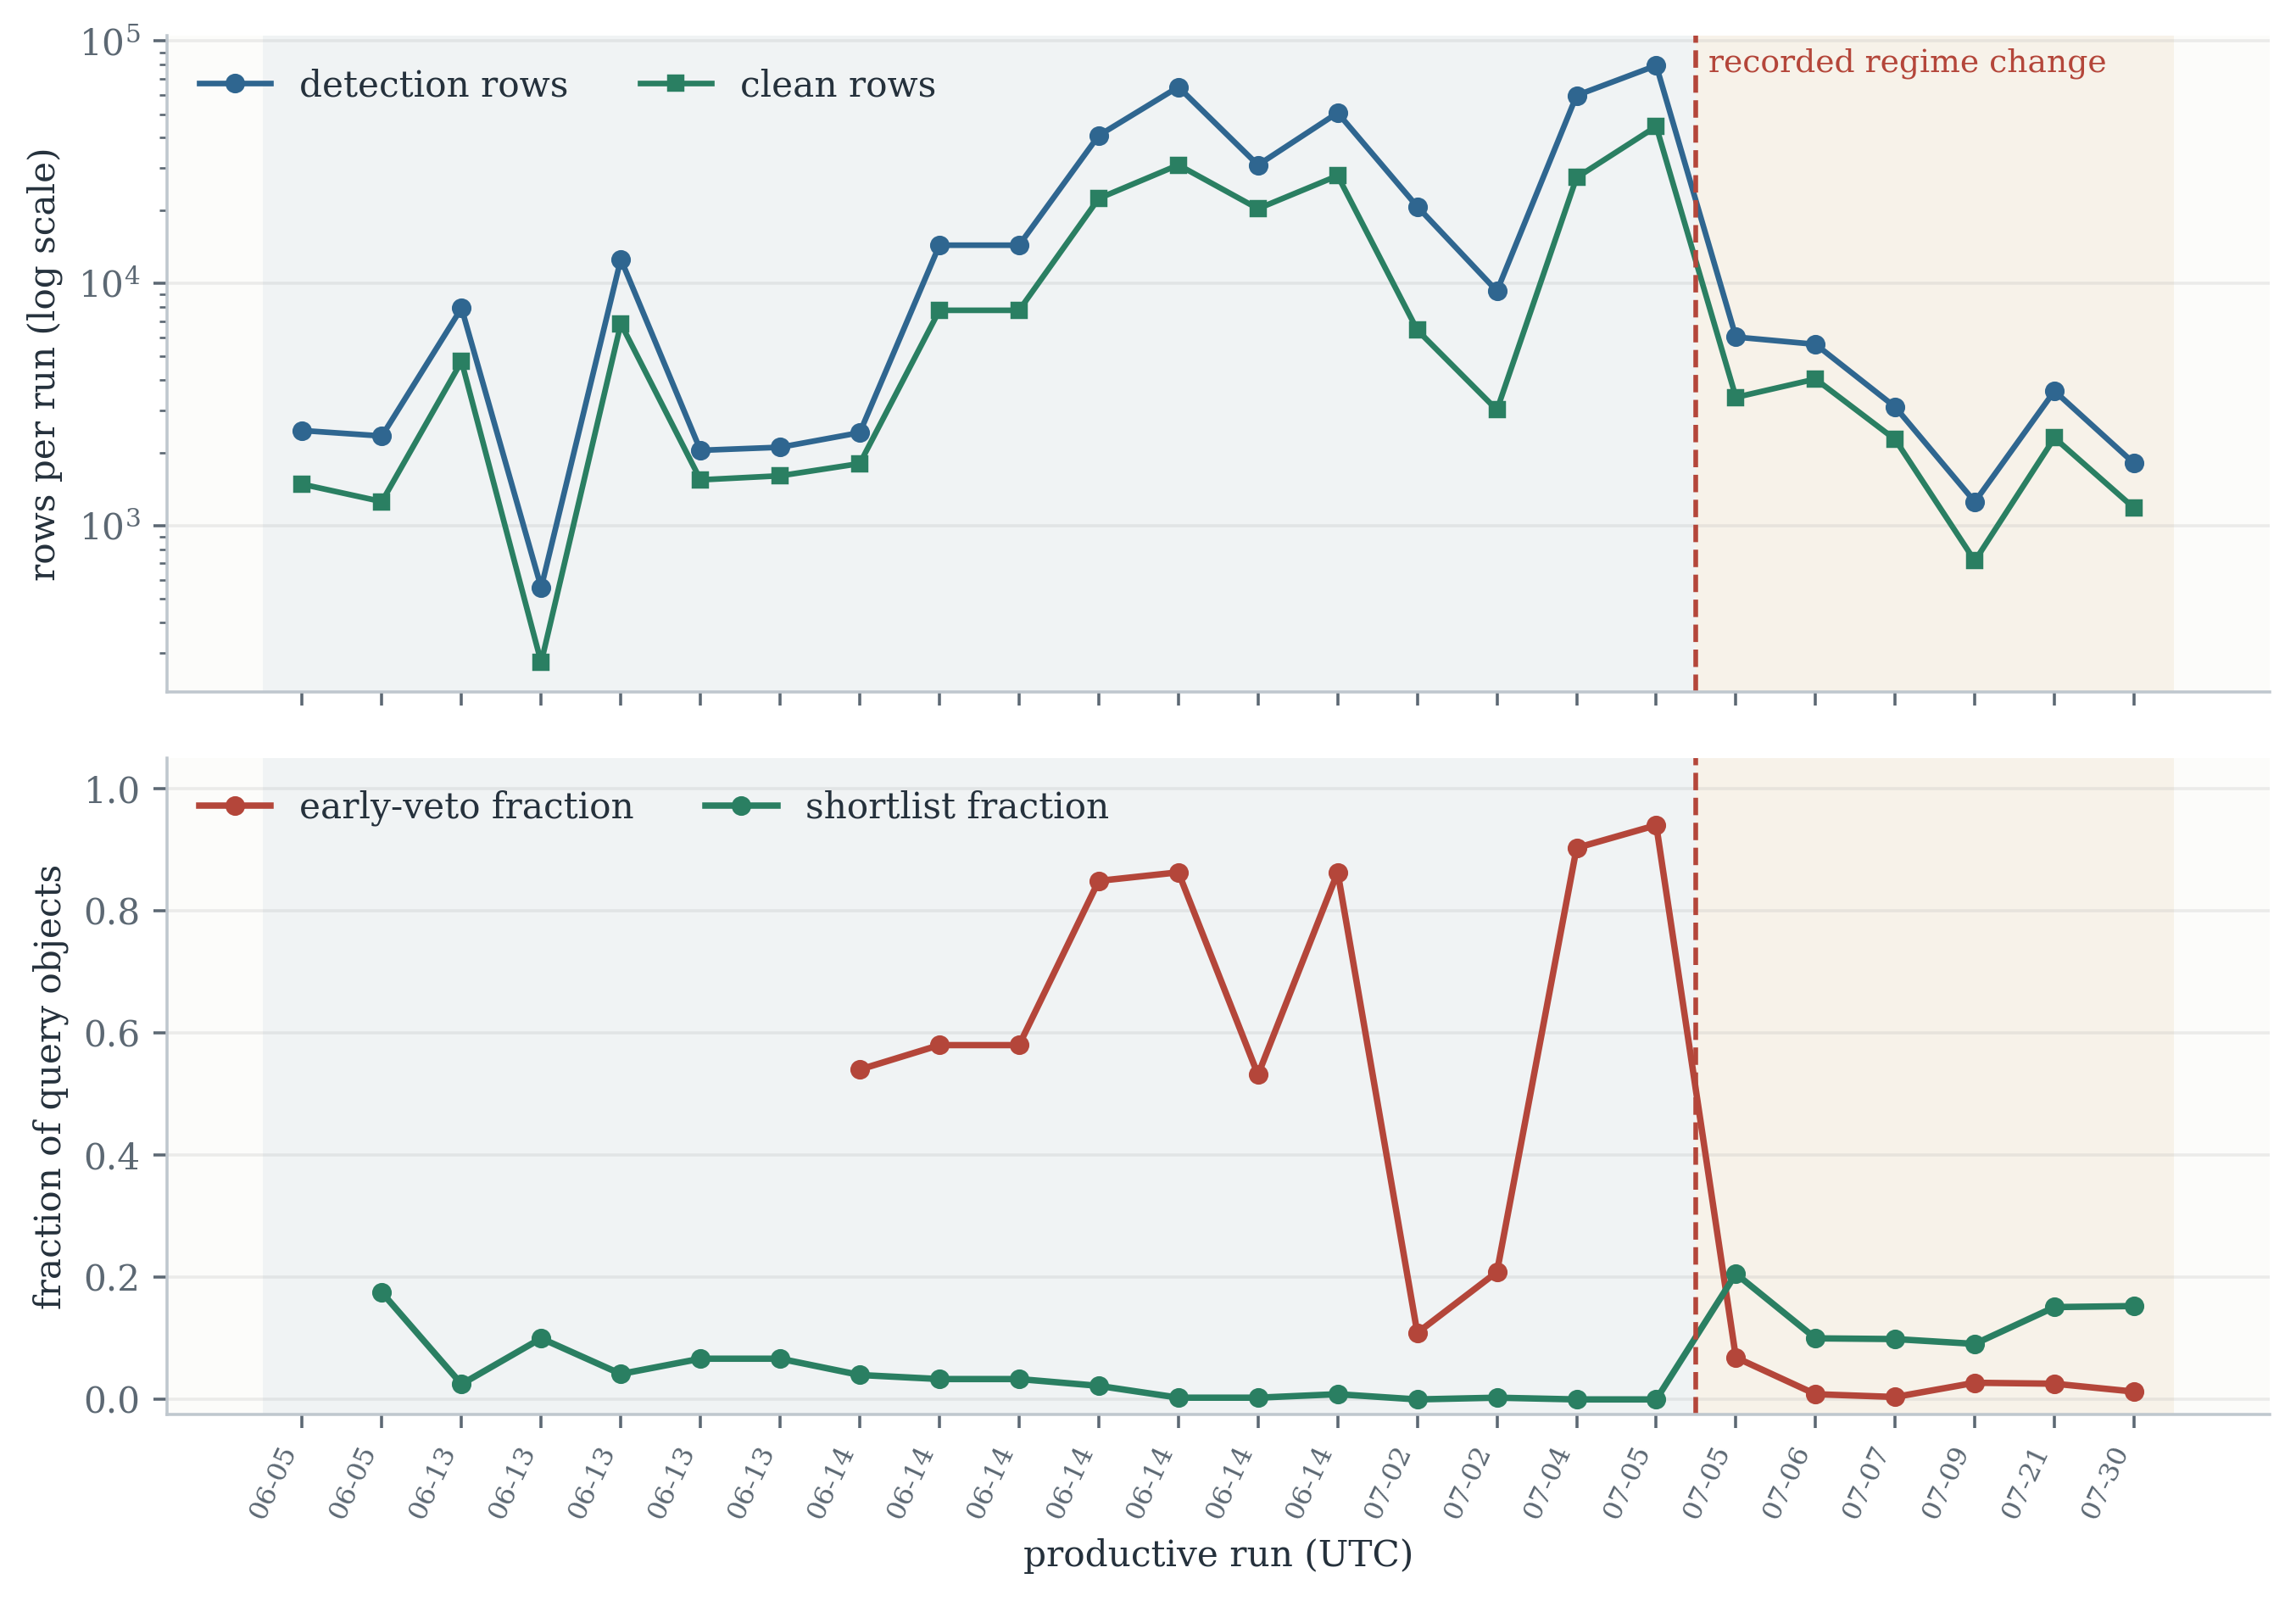
\includegraphics[width=\linewidth]{figures/campaign_dynamics.png}
\caption{Campaign dynamics across productive run records. Top: detection and clean-row workload on a logarithmic scale. Bottom: early-veto and shortlist fractions relative to query-object evaluations. The dashed boundary is descriptive and follows the recorded discontinuity; it is not a statistically estimated change point.}
\label{fig:campaign-dynamics}
\end{figure}

The object evaluations within a run share a query, date, configuration, and upstream service state, so a binomial interval that treats all evaluations as independent would be artificially narrow. We therefore performed a nonparametric cluster bootstrap with productive run as the resampling unit: within each regime, runs were sampled with replacement, their numerators and denominators were summed, and the pooled ratio was recomputed for 50,000 draws using a fixed seed. Figure~\ref{fig:regime-bootstrap} shows percentile intervals. The early-veto change was $-0.518$ with a 95\% run-cluster interval of $[-0.812,-0.282]$; the shortlist change was $+0.134$ with interval $[0.098,0.171]$. The wide pre-retune early-veto interval reflects real run heterogeneity. Neither interval has a causal interpretation because regime assignment is perfectly confounded with calendar time and an undocumented configuration change.

\clearpage
\begin{figure}[h!]
\centering
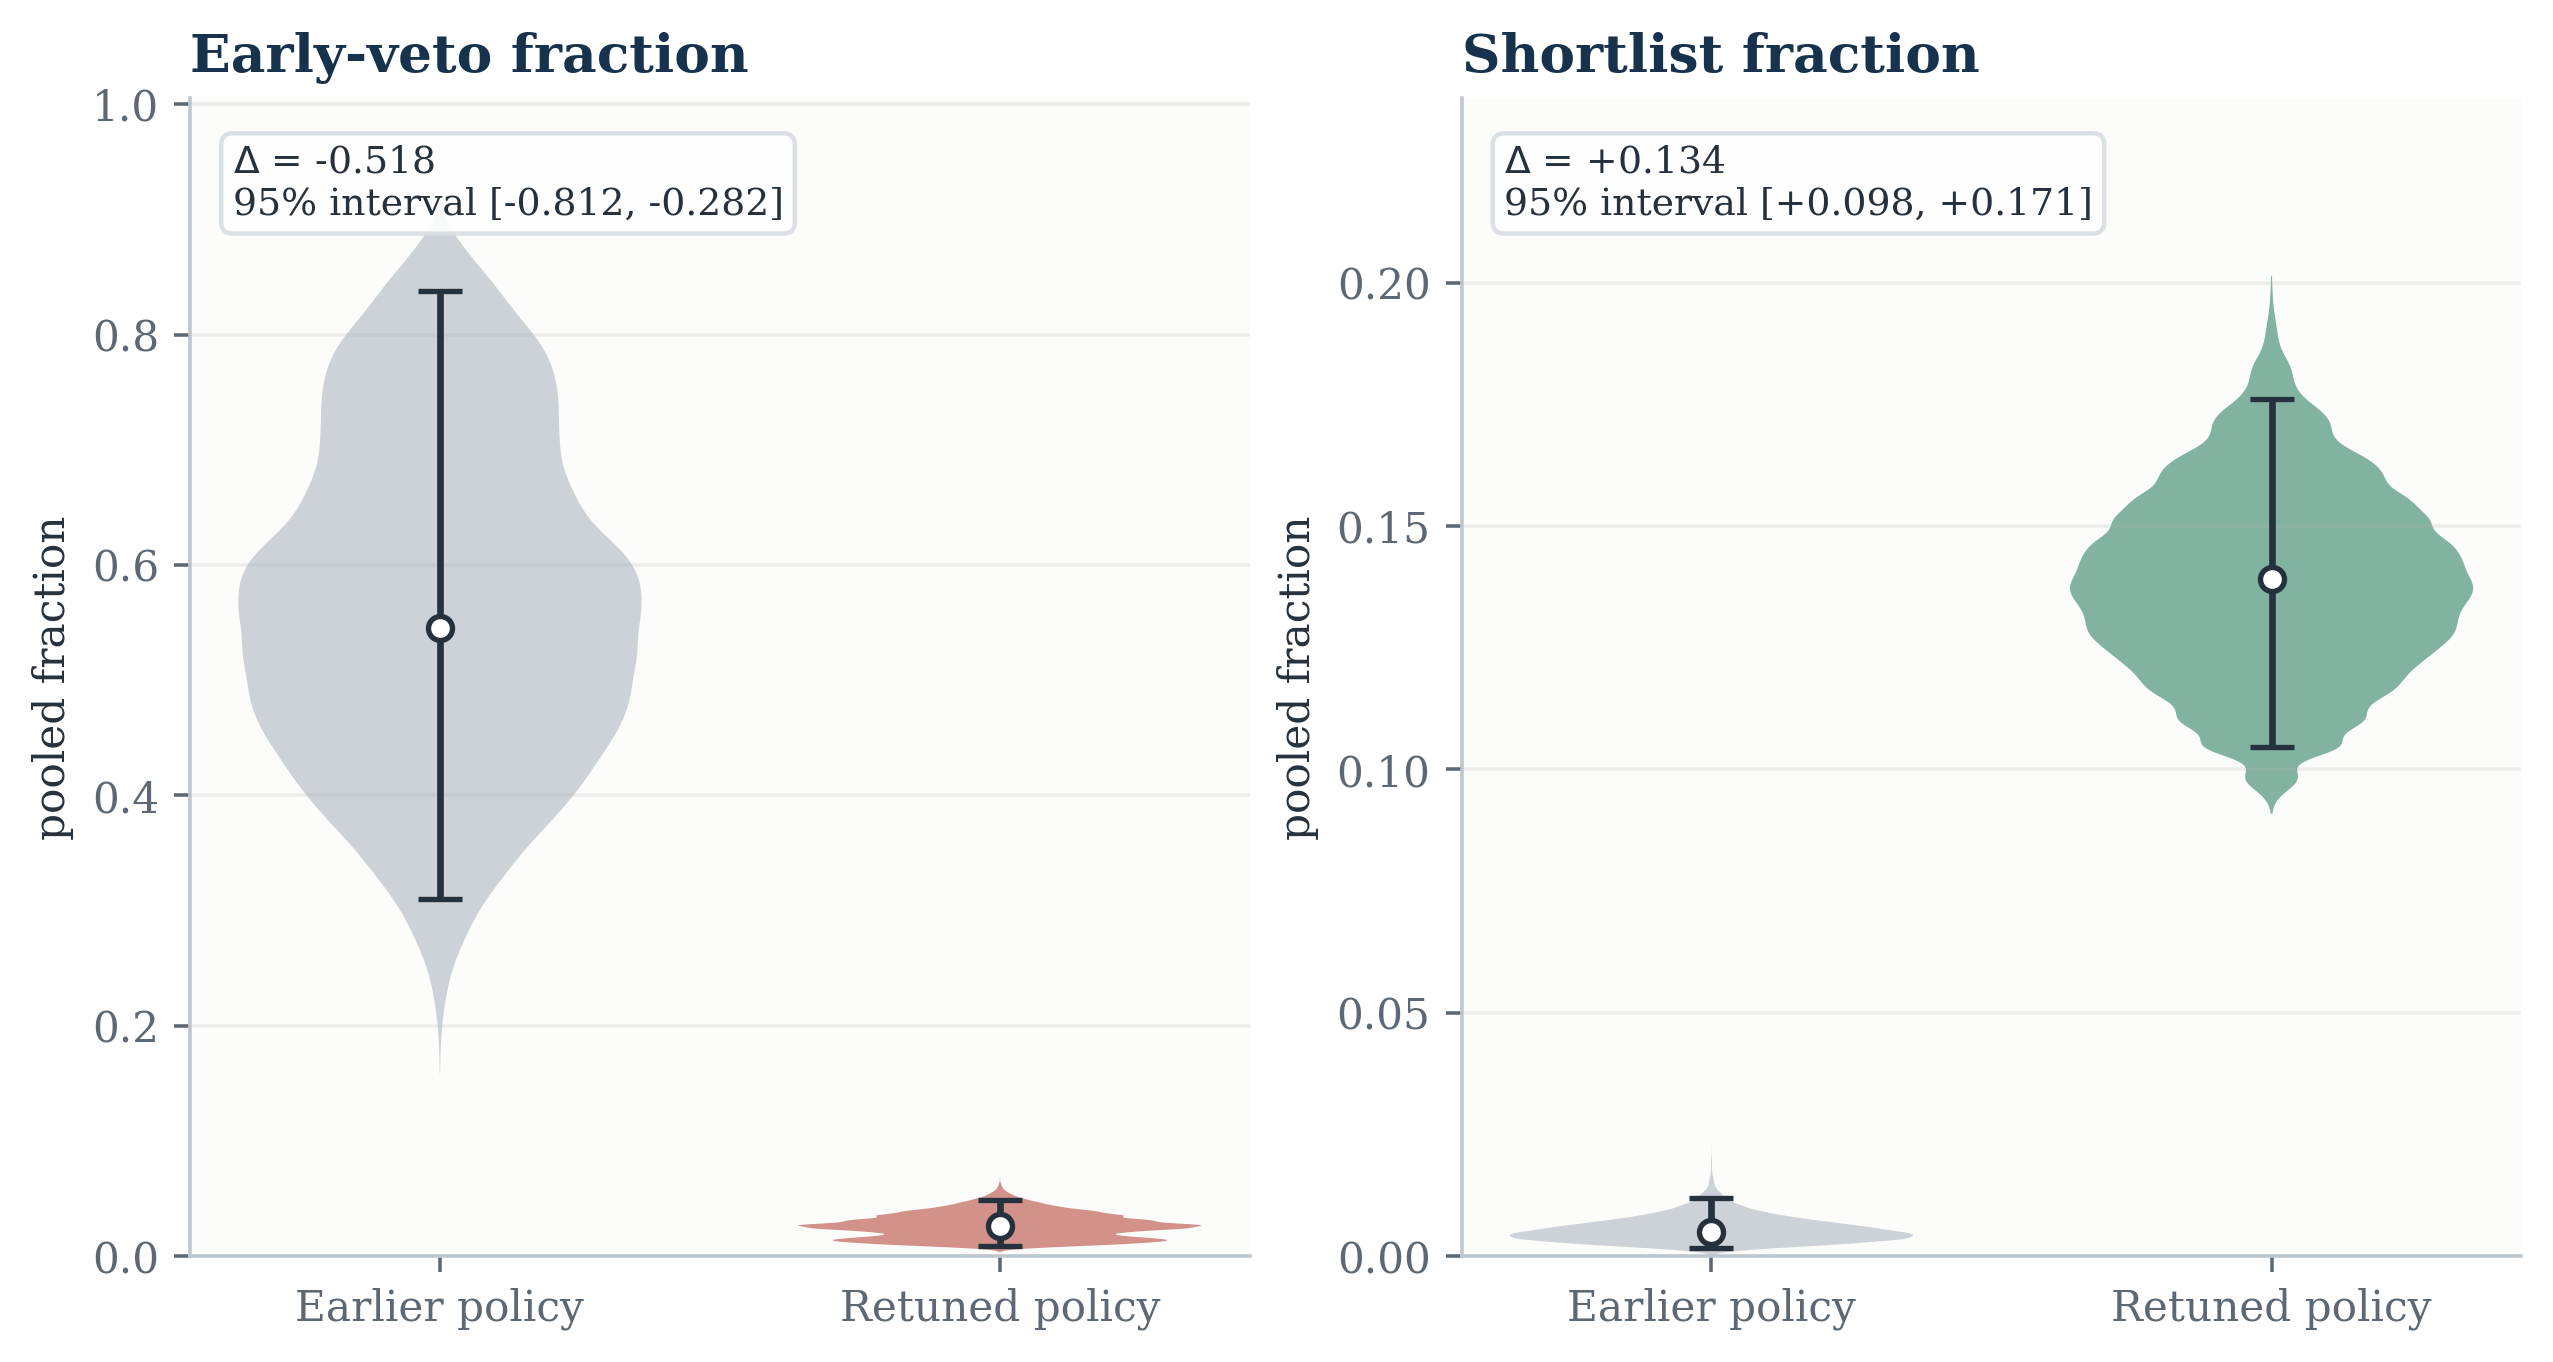
\includegraphics[width=\linewidth]{figures/regime_bootstrap.png}
\caption{Pooled pre- and post-retune fractions with 95\% percentile intervals from a 50,000-draw cluster bootstrap over productive runs. Resampling whole runs preserves within-run dependence. These intervals summarize recorded run-to-run heterogeneity; they are not uncertainty intervals for an astrophysical rate or an identified causal policy effect.}
\label{fig:regime-bootstrap}
\end{figure}

\subsection{Stage-specific rejection accounting}

Table~\ref{tab:funnel} reports the best-supported downstream counts after deduplicating known reprocessing of the same candidate set. Verification included 200 candidate evaluations. Thirty were already known to TNS, none matched a moving object in SkyBoT, and three remained unresolved because TNS queries failed twice. Catalog validation included 193 candidate evaluations: 55 were rejected as known or suspected variables, 30 required manual review, seven were marked as possible host/extragalactic associations, and 101 passed the catalog checks.

The table is \emph{not} a survival curve. The verification and catalog modules do not share an archived row-level cohort in the repository, and the upstream 256 high-priority evaluations include repeated processing. Therefore, subtraction between stage totals would create fictitious attrition counts. Each fraction uses only the denominator shown for its own module.

\begin{table}[ht]
\centering
\caption{Downstream rejection accounting. Counts are candidate evaluations. Categories shown within the catalog module are mutually exclusive; unlisted verification evaluations include candidates that were cleared or had other recorded states.}
\label{tab:funnel}
\begin{tabular}{lrr}
\toprule
Stage/outcome & Count & Fraction within module \\
\midrule
Verification checks & 200 & --- \\
\quad Known TNS object & 30 & 15.0\% \\
\quad SkyBoT moving-object match & 0 & 0.0\% \\
\quad Unresolved TNS status & 3 & 1.5\% \\
\midrule
Catalog-validation checks & 193 & --- \\
\quad Known/suspected variable rejected & 55 & 28.5\% \\
\quad Manual catalog review & 30 & 15.5\% \\
\quad Possible host/extragalactic source & 7 & 3.6\% \\
\quad Passed catalog checks & 101 & 52.3\% \\
\bottomrule
\end{tabular}
\end{table}

Known or suspected variables formed the largest recorded downstream rejection category, with 55 cases. These evaluations had survived broker selection and local light-curve ranking; without catalog validation they could have been advanced as plausible new transients. The 30 TNS matches were candidates already represented in the registry and therefore unavailable for a new discovery report. The absence of SkyBoT matches should not be interpreted as a measurement of Solar System contamination in ZTF. The broker classes and freshness constraints preconditioned the evaluated subset, and multi-epoch stationarity was later required.

\subsection{Descriptive finite-count uncertainty}

To communicate the scale of finite-count variation, we calculate two-sided 95\% Wilson score intervals. For $k$ outcomes in $n$ evaluations, $\hat p=k/n$, and $z=1.96$, the interval is
\begin{equation}
\frac{\hat p+z^2/(2n)\ \pm\ z\sqrt{\hat p(1-\hat p)/n+z^2/(4n^2)}}{1+z^2/n}.
\label{eq:wilson}
\end{equation}
Known-variable rejection was 28.5\% (55/193; Wilson interval 22.6--35.2\%), and known-TNS rejection was 15.0\% (30/200; 10.7--20.6\%). Zero SkyBoT matches among 200 evaluations corresponds to an upper Wilson limit of 1.88\%, not proof of a zero rate.

These intervals are descriptive, not population confidence intervals. The IID binomial assumptions are violated by targeted broker intake, possible repeated objects, configuration changes, and stage-dependent missingness. We include them to prevent small counts from being read with false precision, while explicitly declining inference to the parent ZTF stream.

\subsection{Yield definitions}

Two objects were submitted and assigned TNS designations, AT~2026pcz and AT~2026rsp. Relative to 3,824 distinct screened objects, the submitted-and-designated fraction is
\begin{equation}
  f_{\rm designated} = \frac{2}{3824} = 5.23\times10^{-4} = 0.052\%.
\end{equation}
Only AT~2026rsp has a complete surviving case record in the present repository that supports a credited-discovery statement. The corresponding conservative discovery yield is
\begin{equation}
  f_{\rm discovery} = \frac{1}{3824} = 2.62\times10^{-4} = 0.026\%.
\end{equation}
The Wilson intervals are 0.014--0.191\% for the submitted-and-designated fraction and 0.0046--0.148\% for the single fully preserved credited case. These are operational yields rather than estimates of an astrophysical event rate or classifier precision. The denominator was created by a changing, targeted query and is not a controlled sample of the alert stream. Moreover, ``complete surviving case record'' measures present-day provenance, not necessarily all historical scientific merit.

\section{Representative Candidate Outcomes}
\label{sec:cases}

\subsection{ZTF26abdqbqw = AT 2026rsp}

ZTF26abdqbqw is the campaign's complete positive case. It was first detected at 2026 June 19 10:11:12 UTC at J2000 coordinates $\alpha=22^{\mathrm h}22^{\mathrm m}35.931^{\mathrm s}$, $\delta=+04^{\circ}44'17.77''$. Twenty-three positive detections in $g$, $r$, and $i$ were recorded over 14 nights through 2026 July 3. The object had 36 pre-discovery non-detections, with a best limiting magnitude of 20.551. It brightened by approximately 1.3 mag in ten days and reached approximately $r=19.8$ near 2026 July 1--4.

The position is associated with WISEA J222235.91+044418.8, and the ALeRCE light-curve classifiers favored a Type Ia supernova interpretation. The report nevertheless used unclassified-transient language because no spectrum was available. It was submitted on 2026 July 5 and designated AT~2026rsp (TNS object identifier 212592). An AstroNote requesting spectroscopic classification was published as AstroNote 2026-210 on July 8. The TNS report predates creation of reporting group 204 on July 9 and therefore lists no reporting group; this historical attribution issue should not be propagated to future submissions.

\subsection{ZTF26aascgfc: passed, but not submitted}

ZTF26aascgfc illustrates that a strong candidate need not become a report. It showed seven detections over 3.0 days, from 2026 April 7 to 10, following 61 non-detections reaching a best limit of 20.734 mag. Its brightest recorded measurement was $g=19.947$ on April 9. It had no SkyBoT or TNS match, passed catalog validation, had strong real--bogus metrics, and received a supernova-like stamp label. A report packet was prepared with the decision \texttt{likely\_new\_candidate}, but the operating record contains no submission. Because registry state changes, the historical negative TNS check cannot be treated as current evidence.

\subsection{ZTF26abayrka: a successful wording veto}

ZTF26abayrka had 13 detections over 9.9 days and 50 earlier non-detections, with a best limit of 20.851 mag. A NED galaxy, WISEA J153855.35+102716.1, lies approximately \SI{0.4}{\arcsec} from the candidate position; faint Gaia DR3 and Pan-STARRS counterparts are also present at a similar separation. The ALeRCE AGN probability was approximately 0.815. The object was therefore held back from supernova wording and treated as nuclear/AGN-like. This case demonstrates why host geometry and classifier context must be considered together: a clean, compact residual is not sufficient to identify an explosive transient.

\subsection{Incomplete and stale cases}

The record lists AT~2026pcz as a second submitted and designated object, associated with TNS report 308376, but does not preserve enough object-level metadata to reconstruct a publication-quality case study. We therefore count it in the submitted-and-designated yield but do not present it as the campaign's credited discovery.

A bulk draft prepared on 2026 July 10 contained ZTF26abbkkey, labeled PSN with 40 detections, and ZTF26abboood, labeled NUC with 20 detections. Both were marked \texttt{likely\_new\_candidate} and had no TNS match at draft time, but neither has a recorded submission outcome. Their negative registry checks are stale and must be repeated before any action. Three additional objects from the July 21 run remain unadjudicated after repeated TNS query errors.

\section{Software Verification and Reproducibility}
\label{sec:software-verification}

We completed local technical verification of the current \siderea\ implementation on 2026 September 8 using Python 3.11. Table~\ref{tab:software-verification} distinguishes implementation evidence from scientific validation. The current suite completed 405 tests without failure; strict static typing covered 74 source files, and branch-aware coverage was 78.35\%. Historical multi-interpreter results describe an earlier revision and are archived separately. These checks verify implemented invariants and failure behavior, not astronomical discovery performance.

\begin{table}[ht]
\centering
\caption{Local technical-verification results. Passing these checks establishes software behavior on the tested fixtures, not performance on a representative alert stream.}
\label{tab:software-verification}
\begin{tabular}{p{0.33\linewidth}p{0.18\linewidth}p{0.38\linewidth}}
\toprule
Check & Result & Scope and interpretation \\
\midrule
Unit/invariant suite & 405 tests + 96 subtests passed & Configuration, ingestion, photometry, scoring, clients, evidence binding, ledgers, review, baseline, JEPA, and command behavior. \\
Static analysis & Passed & \texttt{ruff} over \texttt{src} and \texttt{tests}; strict typing over 74 source files. \\
Deterministic local replay & 2/2 fingerprints identical & Same frozen input and scientific policy; distinct execution identifiers. \\
Core artifact identity & 3/3 byte-identical & Normalized photometry, band-aware features, and ranking table. \\
Candidate identity & 2/2 versions identical & Pending-check timestamps differ, but are excluded from scientific identity. \\
Fail-closed fixture & 0/2 reportable & Both candidates blocked because all four mandatory services were pending. \\
Live astronomy services & Not qualified here & Offline adapter tests do not establish current live behavior or prospective performance. \\
\bottomrule
\end{tabular}
\end{table}

Two executions of the checked-in \texttt{examples/photometry.csv} fixture produced the same scientific fingerprint, \texttt{analysis-7d203c8f40012eb4}. Their normalized tables, feature tables, and rankings were byte-identical, and both candidate-version digests agreed. The candidate envelopes and manifests were intentionally not byte-identical because they record execution-specific run identifiers and pending-check timestamps. This separation is the intended behavior of Equation~\ref{eq:candidate-version}: reproducibility means identical scientific state, not deletion of execution provenance.

The same replay produced two candidates, both blocked and neither reportable, because SkyBoT, TNS, SIMBAD, and VSX evidence remained pending. This is a positive safety test: the local score and deterministic ranking completed, yet absence of network evidence did not become clearance. Conversely, this audit did not perform a live ALeRCE fetch, catalog query, image-level review, multi-user review study, or TNS submission. The verified maturity is therefore implementation-level and fixture-level, below retrospective benchmarking on a frozen representative alert cohort.

Tiny synthetic execution checks also exercised the logistic baseline and JEPA training paths. The baseline retained an uncalibrated-score label because its three-row calibration partition could not supply the required five examples per class. A three-epoch JEPA run and repeated-mask evaluation exercise checkpointing and numerical execution only; they do not demonstrate useful representations or astronomical generalization. The full smoke metadata is retained in \texttt{paper/experiments/learning-smoke-results.json}.

\section{Synthetic Transient-Search Diagnostic}
\label{sec:synthetic-search}

The operational audit motivated a shadow-only detection experiment: can evidence
spread across irregular flux measurements improve excess detection relative to a
single-epoch statistic while accounting for unknown peak time? We implemented four
nonnegative, unit-peak shapes: Gaussian, asymmetric exponential, Bazin
\citep{bazin2009}, and a Gaussian rise joined to a $(1+\Delta t/w)^{-5/3}$ tail.
The Bazin and exponential shapes fix the fall-to-rise timescale ratio at three.
These are phenomenological morphology templates, not explosion simulations or
unique physical-class identifiers. Debris fallback need not trace optical luminosity,
and partial disruptions can show different asymptotic behavior \citep{miles2020}.
Timescales are in the observer frame.

For flux $y$, template $h$, background $b$, amplitude $A\geq0$, and declared
covariance $C=LL^\top$, the model is $y=b\mathbf{1}+Ah+\epsilon$ with
$\epsilon\sim\mathcal{N}(0,C)$. Writing $u=L^{-1}\mathbf{1}$ and
$q=(I-uu^\top/(u^\top u))L^{-1}h$, the profiled statistic is
\begin{equation}
z_h=\frac{q^\top L^{-1}y}{\sqrt{q^\top q}},\qquad
T=\max_{h\in\mathcal H}\max(0,z_h).
\end{equation}
The local likelihood improvement is $\Delta\chi^2=\max(0,z_h)^2$; it does not
provide a chi-square calibration for the bank maximum. Each null simulation
repeats the entire search, giving the finite Monte Carlo p-value
\begin{equation}
\widehat p(T)=\frac{1+\sum_{j=1}^{N_0}\mathbf{1}[T_j^{(0)}\geq T]}{N_0+1}.
\end{equation}
Passbands remain separate, with conservative within-object Bonferroni correction.
This does not control all survey objects or repeated monitoring decisions.
Invalid covariance, censored limits masquerading as flux, and ill-conditioned
designs are rejected; insufficient-epoch channels remain explicitly unevaluated.

The local design fixes 64 irregular epochs over 60 days, heterogeneous marginal
errors, 21 searched centers, three widths (1, 3 and 10 days) and four families:
252 templates. Each method uses 4,095 calibration curves for a nominal 1\%
per-curve rule and 1,000 evaluation curves per scenario. Injected centers range
from 10 to 50 days and widths are log-uniform from 1 to 10 days, allowing grid
mismatch. The comparator is the maximum positive standardized residual after a
fitted constant, separately calibrated on the same null distribution. Calibration
and evaluation use separate random streams. Methods and amplitudes share test
noise; row-wise Wilson intervals are conditional Monte Carlo intervals, not
independent population confidence statements or a formal superiority test.

\begin{table}[ht]
\centering
\caption{Measured synthetic detections per 1,000 evaluation curves. Pulse rows are recovery; null and outlier rows are false alarms. The last row uses a new seed and supplied covariance.}
\label{tab:search-diagnostic}
\begin{tabular}{p{0.47\linewidth}rr}
\toprule
Scenario & Bank & Single epoch \\
\midrule
Gaussian pulse, 2-sigma peak & 707 & 136 \\
Exponential pulse, 2-sigma peak & 336 & 60 \\
Bazin pulse, 2-sigma peak & 621 & 101 \\
Fallback pulse, 2-sigma peak & 552 & 87 \\
Independent Gaussian null & 13 & 6 \\
AR(1), diagonal calibration & 454 & 4 \\
One positive 8-sigma outlier & 710 & 1000 \\
AR(1), known-covariance calibration & 11 & 3 \\
\bottomrule
\end{tabular}
\end{table}


\begin{figure}[ht]
\centering

\includegraphics[width=\linewidth]{experiments/transient-search-final/search_diagnostic.png}
\caption{Synthetic recovery and false-alarm diagnostic. Solid curves use the
template bank; dashed curves use the separately calibrated single-epoch comparator.
The right panel deliberately violates independent Gaussian calibration. Counts,
marginal intervals and per-trial statistics are archived. These are not survey
completeness measurements.}
\label{fig:synthetic-search}
\end{figure}

The correlated-noise failure motivated an adaptive follow-up with a new seed and
an explicitly supplied AR(1) correlation, $R_{ij}=0.7^{|i-j|}$, used in both
whitening and calibration. This is an oracle-covariance diagnostic, not a survey
noise estimate. The original failure is retained. Isolated outliers remain a
serious limitation, and unknown covariance, seasonal sampling, calibration
systematics and artifacts require representative data and independent image review.
The CLI also offers a declared exponential time-covariance with 80\% correlated
and 20\% independent variance; these hyperparameters are not fitted on the target.
Neither experiment changes heuristic ranking, catalog gates or human approvals.

Protocols, source snapshots, per-trial statistics and plotting code are archived
under \texttt{paper/experiments}. Each design was recorded locally before its run;
the covariance follow-up was designed after the initial failure, not externally
preregistered. Historical campaign counts are unchanged by these simulations.

A second adaptive stress design uses the declared exponential covariance
(six-day timescale, 80\% correlated variance), independent calibration/evaluation
streams, and 1,000 null trials per row. The matched Gaussian case produces
11 false alarms; multiplying the actual standard deviations by 1.5 while retaining
the quoted errors produces 337. Unit-variance Student-$t_3$ innovations propagated
through the correlation factor produce 104, and doubling the variance after day 30
produces 118. A seasonal gap with correctly matched calibration produces 10;
true correlation timescales of one and 20 days, while assuming six days, produce
129 and two, respectively. All seven rows, their marginal Wilson intervals and
trial statistics are retained in \texttt{noise-stress-final}. These results show
that a supplied covariance is insufficient when noise assumptions are wrong;
they neither estimate real survey false-alarm rates nor measure recovery across
these stress conditions. No threshold was retuned using these outcomes.


\section{Discussion}
\label{sec:discussion}

\subsection{Interpretation of rejections}

The campaign applied restrictive triage. Its surviving record contains one fully documented credited case among 3,824 screened objects. The same record contains 55 variable-star rejections and 30 pre-existing TNS matches, showing that a high-priority broker candidate was not necessarily a novel reportable event. The broker classifier and local features address whether an object resembles a transient; the downstream catalogs address known-source associations; TNS records whether the object was already reported; and stamp review addresses whether the signal was morphologically credible. These are distinct hypotheses.

The same principle applies to nuclear events. A transient coincident with a galaxy can be scientifically valuable, but an elevated AGN probability and sub-arcsecond nuclear association demand different wording from an off-nuclear supernova candidate. The pipeline's purpose is not to force every survivor into a supernova category; it is to preserve an auditable relationship between evidence and claim.

Classifier performance, novelty, reportability, registry acceptance, and physical classification have different truth conditions. A source can be correctly labeled ``SN-like'' by a broker yet be non-novel because another group reported it first. It can be novel and astrophysically real yet non-reportable under the project's policy because its evidence is stale or no independent reviewer is available. It can be designated by TNS and later prove to be a variable. No single scalar accuracy summarizes these outcomes.

\subsection{Interpretation of stage counts}

The catalog result directly establishes that 55 recorded evaluations were stopped by a rule for known or suspected variables. It does not establish that all 55 would otherwise have been submitted, that every match is physically correct, or that the remaining 138 were non-variable. Similarly, the 30 TNS matches establish a duplicate-reporting veto, not the astrophysical purity of either the matched or unmatched subset.

An ablation study would be required to estimate each gate's marginal contribution. For example, replaying the same frozen cohort with and without VSX could measure how many manual reviews, packets, and false reports the VSX gate changes. Replaying without the age and history vetoes could quantify whether they mostly remove known variables or also suppress real supernovae. AMPEL's comparison of more than 200 selection functions provides a precedent for this kind of alert replay \citep{nordin2019}. The present archive lacks the complete row-level cohort and negative outcomes needed to perform those ablations honestly.

The apparently large difference between 3,824 distinct retrieved objects and one fully preserved credited case should therefore not be called a false-positive rate. Most retrieved objects were never asserted to be positive examples, and rejected objects lack exhaustive truth labels. Likewise, there is no false-negative rate because the project did not revisit all rejected positions after a fixed maturation period to identify missed TNS transients.

\subsection{Human judgment and reproducibility}

Image-level review remains necessary because scalar features do not capture all subtraction failures. The protocol makes this judgment more reproducible by specifying a fixed panel order, requiring consistent residuals on at least two dates, and recording explicit failure patterns. This resembles the automatic-filter-plus-expert-scanning pattern used by ALeRCE SN Hunter and ZTF BTS \citep{carrascodavis2021,fremling2020}. It remains weaker than a measured review process because only one operator's labels survive. A prospective study should present a common blinded set to two reviewers, record rejection reasons independently, and report both raw agreement and a chance-corrected statistic.

Failed external queries are represented as unresolved states rather than silently converted to non-matches. This distinction proved material: three candidates remained blocked after two TNS failures. In reliability terms, this is fail-closed behavior. It reduces the risk of duplicate reporting at the cost of delaying or missing time-sensitive candidates when dependencies are unavailable. Both outcomes should be measured: query completion rate and time-to-clear belong beside astronomical yield.

Both the historical score and the \siderea\ decomposition are intentionally inspectable. Their coefficients are heuristics, not outputs of training or probability calibration. The \siderea\ implementation improves measurement semantics and exposes each component and warning, but transparency does not establish optimality. A future labeled set of accepted transients, known variables, artifacts, and missed opportunities would allow threshold tuning and comparative evaluation without sacrificing the rule-based safety gates.

\subsection{Crossmatch asymmetry and host ambiguity}

Catalog matching creates two opposing risks. A radius that is too small misses true counterparts; a radius that is too large rejects candidates because of unrelated neighbors. The probability of chance coincidence increases with local catalog density, so a single \SI{3}{\arcsec} threshold has different meaning at high and low Galactic latitude. Proper motion further complicates stellar matches when catalog and alert epochs differ. A posterior association model should combine separation normalized by the joint astrometric covariance with local density and object-type priors \citep{budavari2008}. Until then, \legacycampaign's conservative catalog veto protects reporting precision but has an unknown completeness cost.

Host association is still more nuanced. A close galaxy match can support an extragalactic origin while a nuclear offset can raise the probability of AGN variability or a tidal disruption event. Angular separation alone is not a physical offset without a distance, and a nearest catalog source is not necessarily the host. ZTF BTS demonstrates that host-catalog incompleteness itself varies with galaxy brightness and redshift \citep{fremling2020}. The \legacycampaign\ wording gate is therefore a claim-control mechanism, not a host-classification algorithm.

\subsection{Operational implications}

The historical campaign relied on an exclusion ledger, run summaries, and post-submission records, but configuration changes and several candidate outcomes were not archived completely. \siderea\ adds versioned policy identifiers, machine-readable evidence states, independent review, and explicit outcome closure. The local verification in Section~\ref{sec:software-verification} tests these mechanisms but does not establish that live services will meet their assumed contracts or that the procedures will be followed consistently during observing operations.

Broker ingestion and enrichment need not be reproduced by a small reporting program. The downstream task is to define a science policy, allocate limited review time, and record the disposition of each reviewed candidate. Evaluation should therefore include review load, service availability, latency, duplicate-report rate, and claim accuracy in addition to ranking performance.

\section{Limitations}
\label{sec:limitations}

\subsection{Cohort and provenance}

The historical search was restricted to selected supernova-like broker classes and did not preserve a closed row-level cohort. Some objects were processed more than once, and the stage tables cannot be joined into a complete object-level history. The 3,824 cached object identifiers provide the best unique denominator; sums of run-level row counts are workload measures and can include reprocessing. The record for AT~2026pcz is incomplete, the July 10 bulk draft has no final disposition, and three July 21 candidates retain unresolved TNS status.

The operating policy also changed during the campaign. On July 5, the recorded early-veto count fell from 329 to 24 between adjacent productive runs and the shortlist increased from zero to 72. The exact configuration change was not archived. Calendar time, input population, and policy version are consequently confounded, so the cluster bootstrap quantifies run-to-run variation but not the causal effect of the change.

\subsection{Measurements and ranking}

The legacy feature calculation pooled $g$, $r$, and $i$ magnitudes. Differences in color and filter cadence can therefore affect the estimated scatter, amplitude, significance, and periodicity. Recency was measured relative to the newest detection in the fetched batch rather than to an absolute query time, which makes the score dependent on other objects in the batch. The score coefficients were set by hand, several terms share information, and the broker probability was not recalibrated for the selected population.

No injection--recovery analysis was performed, and rejected objects were not systematically re-evaluated after a fixed maturation interval. The campaign therefore provides no estimate of detection efficiency as a function of magnitude, cadence, host surface brightness, timescale, or transient class, and it does not measure the number of missed transients.

\subsection{External data and human review}

Catalog associations were based on fixed angular radii. Their interpretation depends on catalog completeness, local source density, positional uncertainty, proper motion, and catalog epoch. A completed non-match is not evidence that no counterpart exists, and a nearby match is not necessarily physical. Seven broker-query runs failed, but the archive does not contain systematic service-completion or latency measurements.

The historical image review was performed by one operator, and independent labels were not preserved. The current software requires separate screener and reviewer roles, but retrospective agreement cannot be estimated. TNS designation is a registry result rather than a spectroscopic classification; no spectrum is available in the surviving record for AT~2026rsp.

\subsection{Scope of the implementation audit}

The band-aware feature path, content-addressed evidence, review binding, preflight gate, and shadow-model interfaces belong to \siderea\ and were not used in the historical campaign. The local audit runtime included NumPy, pandas, scikit-learn, PyTorch, and Matplotlib, but not Astropy, astroquery, or the ALeRCE client. The replay therefore verifies local deterministic behavior and blocking under missing evidence, not live broker or catalog integration. TS-JEPA, feature-space anomaly scoring, and the supervised baseline have not been compared with the heuristic on an object-grouped chronological cohort.

\section{Prospective Evaluation}
\label{sec:validation}

The next campaign should freeze a configuration in a versioned run manifest and record the code revision, query timestamps, catalog service status, model/classifier names, and every threshold. Each stage should emit an immutable row-level table keyed by object identifier and evaluation timestamp. The submission log should record the screener, reviewer, wording, TNS report identifier, final designation, and confirmation method. Automated retry and alerting should distinguish service failures from valid zero-result queries.

\subsection{Outcome definitions}

A single label such as ``good candidate'' is insufficient. The benchmark should record at least four axes: (1) real versus subtraction artifact; (2) stationary versus moving; (3) novel versus already registered at the decision timestamp; and (4) best available physical class after a fixed maturation interval. ``Reportable under the \legacycampaign\ policy'' is a derived decision label, not a physical truth class. TNS can provide novelty and later classifications, but absence from TNS is not a complete negative label.

\subsection{Replay cohort and temporal split}

One useful design is a time-bounded, frozen set of all broker objects satisfying the documented ALeRCE query, including those rejected before shortlisting. Outcomes should be frozen after a predetermined delay long enough for independent TNS reports and catalog updates. Threshold development should use an earlier interval and all headline metrics should be computed once on a later, untouched interval. AMPEL's alert reprocessing demonstrates the value of replay for comparing selection functions \citep{nordin2019}; ZTF BTS demonstrates how magnitude and coverage cuts can define a statistical sample with measured spectroscopic completeness \citep{perley2020}.

For a binary policy target, report precision and recall,
\begin{equation}
  \mathrm{precision}=\frac{TP}{TP+FP}, \qquad
  \mathrm{recall}=\frac{TP}{TP+FN},
\end{equation}
along with the precision--recall curve, review fraction, reports per reviewer-hour, and median decision latency. Because the science cost of missing a young transient differs from the cost of delaying a variable, metrics should also be stratified by age at first review, magnitude, number of detections, Galactic latitude, host surface brightness, and physical class. A Fink active-learning study, for example, reported both purity and efficiency on a labeled alert set rather than inferring performance from submitted-candidate yield \citep{leoni2022}.

\subsection{Selection function, audit sampling, and censoring}

Let $\theta$ denote a vector of physical and observational parameters---peak magnitude, timescale, color evolution, sky background, cadence, and host offset---and let $x$ denote the realized alert data. For a frozen policy $\pi$, the end-to-end reporting selection function is
\begin{equation}
  \epsilon_{\pi}(\theta)=
  \int \mathrm{I}\!\left\{\pi(x)=\text{report}\right\}
  p(x\mid\theta)\,\mathrm{d}x.
\label{eq:selection-function}
\end{equation}
This integral includes upstream alert generation, broker ingestion, missing services, pipeline gates, and human review. Computing only the software-stage acceptance probability would condition away earlier losses and would not support an astrophysical rate correction.

Complete outcome labeling may be too expensive for every rejected object. If object $i$ is selected for retrospective adjudication with known probability $\pi_i^{\rm audit}>0$, a design-based estimate of an outcome mean can use the H\'ajek form
\begin{equation}
  \widehat{\mu}_{\rm H}=
  \frac{\sum_i A_iY_i/\pi_i^{\rm audit}}
       {\sum_i A_i/\pi_i^{\rm audit}},
\label{eq:hajek}
\end{equation}
where $A_i$ indicates completed audit and $Y_i$ is a frozen terminal outcome. This estimator requires the sampling probabilities to be logged and cannot repair convenience sampling with unknown inclusion probabilities.

Decision latency is right-censored when a candidate remains blocked or unresolved at campaign close. For event times $t_k$, event counts $d_k$, and risk sets $n_k$, a nonparametric summary is the Kaplan--Meier estimator
\begin{equation}
  \widehat{S}_{\tau}(t)=\prod_{t_k\leq t}\left(1-\frac{d_k}{n_k}\right),
\label{eq:kaplan-meier}
\end{equation}
reported separately for rejection, clearance, submission, and unresolved dependency states. Competing outcomes require cause-specific cumulative incidence rather than treating non-submission as a single failure class. The historical record lacks complete timestamps for this analysis; Equations~\ref{eq:selection-function}--\ref{eq:kaplan-meier} define the data contract for the prospective campaign.

\subsection{Injection, recovery, and ablation}

Injection--recovery should sample event amplitude, rise and decline time, color evolution, limiting magnitude, cadence, missing bands, pre-discovery non-detections, and host background. Light-curve-level injection can test ranking logic, but image-level injection is required to measure losses in subtraction and stamp review. HiTS provides a precedent for combining empirical limiting-magnitude distributions with injected supernova light curves to estimate recovery \citep{forster2016}.

Every safety gate should also be ablated on the frozen cohort: broker-probability threshold, pooled versus per-band features, period veto, age/history vetoes, TNS, SkyBoT, VSX, SIMBAD, and human stamps. Report the incremental change in true positives, false positives, review load, and latency. This would reveal whether the 28.5\% catalog rejection fraction represents unique value from VSX/SIMBAD or contamination already predictable from upstream features.

\subsection{Calibration, association, and reviewer reliability}

If $Q$ is retained only for ordering, rank metrics and yield-versus-review-budget curves are sufficient. If it is ever called a probability, it must be calibrated prospectively with reliability diagrams, Brier score, and calibration error on the deployment population. Broker-class probabilities should be assessed separately from the composite score.

Fixed-radius associations should be replaced or supplemented with the Bayes factor for a shared source, using positional covariances and local background density \citep{budavari2008}. Manual review should be duplicated blindly for a stratified sample, with disagreements adjudicated only after independent labels are saved. Raw agreement, class-specific agreement, and a chance-corrected statistic should be reported together with review time.

\subsection{Shadow-model and top-$K$ evaluation}

The learned routes should first run in shadow mode beside the heuristic without changing eligibility or reportability. For night $n$, method $m$, and a frozen review budget $K$, let $Y_{nm}(K)$ be the number of terminally useful candidates within the first $K$ reviewed objects and $T_{nm}(K)$ the reviewer minutes consumed. The primary paired contrast should be
\begin{equation}
  \Delta_Y(K)=\frac{1}{N}\sum_{n=1}^{N}
  \left[Y_{n,\mathrm{new}}(K)-Y_{n,\mathrm{baseline}}(K)\right],
\label{eq:paired-topk}
\end{equation}
with a corresponding time-normalized contrast and a night-block confidence interval. This aligns evaluation with the actual finite queue and avoids converting anomaly or embedding scores into pseudo-probabilities. The comparison should include the heuristic, broker score, supervised logistic baseline, feature-space anomaly model, TS-JEPA, and the same downstream head without TS-JEPA embeddings.

Different anomaly routes should be evaluated both jointly and separately. For routes $r$ and $s$, report overlap $J_{rs}=|\mathcal{Q}_r\cap\mathcal{Q}_s|/|\mathcal{Q}_r\cup\mathcal{Q}_s|$, unique useful yield, and corruption rate. The low route overlap reported by AHA indicates that complementarity can be scientifically useful \citep{iskandarli2026}; it can also mean that one representation is selecting artifacts. StarEmbed, AstroCo, and Astra-CLR provide relevant representation baselines, but their published tasks and populations differ from reportable-transient triage \citep{li2026,tan2025,majumder2026}. Promotion therefore requires an object-grouped, chronological, in-domain comparison rather than citation-level analogy.

\subsection{Registered change control and safety non-inferiority}

Every scientific-policy edit should create a new immutable policy identifier before it receives outcomes. A shadow comparison may run policies in parallel on the same immutable input, but only the preregistered incumbent can drive action. Promotion should require both superiority on the primary top-$K$ yield endpoint and non-inferiority on safety endpoints such as duplicate escape, known-variable escape, and fraction of reportable decisions lacking fresh evidence. If $p_{\rm new}$ and $p_{\rm old}$ are safety-event rates, a one-sided requirement is
\begin{equation}
  \sup \mathrm{CI}_{1-\alpha}\!\left(p_{\rm new}-p_{\rm old}\right)<\delta_{\rm safe},
\label{eq:safety-noninferiority}
\end{equation}
where $\delta_{\rm safe}$ is fixed before evaluation. A threshold or feature changed after examining test outcomes starts a new evaluation interval. This prevents the configuration discontinuity documented in the legacy campaign from recurring as an untraceable mixture of policies.

\subsection{Outcome closure}

Target follow-up should be treated as part of the state machine rather than an informal afterthought. For candidates near peak, a designation should trigger a timestamped AstroNote or direct classification request, visibility estimates, and closure of the outcome record. Every external response should be stored with query time and service version where available. Only then can the analysis distinguish an astronomical rejection from a service outage or an operator delay.

\subsection{Pre-registered decision analysis}

The next evaluation should pre-register the parent interval, query, thresholds, required services, outcome-maturation delay, primary metric, and exclusion rules before the test interval begins. A useful primary operational endpoint is precision among submitted reports under a fixed reviewer-hour budget; a co-primary safety endpoint is duplicate-report rate. Recall among broker-eligible, subsequently confirmed transients can be estimated only after reconstructing every eligible object in the frozen interval. Any threshold changed after inspecting test-period outcomes should define a new policy version and a new evaluation interval rather than being pooled into the original result.


\section{Conclusions}

We have presented a run-level audit of the \legacycampaign\ campaign and the implementation of its successor, \siderea. The campaign processed 3,824 distinct ALeRCE objects in 24 productive runs. Among the recorded downstream evaluations, 30 of 200 registry checks identified an existing TNS object and 55 of 193 catalog checks identified a known or suspected variable. Two submitted sources received TNS designations; ZTF26abdqbqw = AT~2026rsp is the only case for which the repository contains a complete discovery record.

The run summaries also show a substantial policy discontinuity on 2026 July 5. The early-veto fraction decreased from 54.5\% to 2.68\%, while the shortlist fraction increased from 0.51\% to 13.9\%. Cluster-bootstrap intervals describe the between-run variation in these quantities, but the change cannot be attributed causally because policy version, date, and query composition are confounded.

\siderea\ addresses the provenance and state-management weaknesses found in the campaign record. Candidate versions are content-addressed; external results are bound to position, epoch, radius, and lifetime; review decisions apply to a specific candidate version; and report preparation requires every mandatory clearance. The current implementation passed 405 tests on Python 3.11 and reproduced the scientific outputs of the local replay fixture. A time-forward object-level cohort, complete outcomes, injection--recovery tests, and independent review labels are still required to estimate completeness or compare ranking methods.

\section*{Acknowledgments}

This work makes use of data from the Zwicky Transient Facility. ZTF is supported by the National Science Foundation and an international collaboration of partners. This research used the ALeRCE broker, the Transient Name Server, the SIMBAD database and VizieR catalog access tool operated at CDS, Strasbourg, the AAVSO International Variable Star Index, the IMCCE SkyBoT service, and NASA/IPAC archival services.

\section*{Data Availability}

The source code, operating protocol, campaign-level audit record, manuscript source, bibliography, and figure-generation program are included with the project. Live-query outputs, cached light curves, candidate shortlists, report packages, and correspondence were intentionally untracked during the recorded campaign. Consequently, the aggregate results can be audited against the surviving summaries, but the exact stage-by-stage cohort cannot be independently reconstructed from the repository alone. Because upstream alert and catalog services evolve, future releases should archive immutable row-level manifests, service responses or content hashes where redistribution permits, configuration files, and final outcome tables.

\section*{Software}

The pipeline uses Python, NumPy \citep{harris2020}, pandas \citep{mckinney2010}, Astropy \citep{astropy2013,astropy2018}, astroquery \citep{ginsburg2019}, Matplotlib \citep{hunter2007}, and the ALeRCE Python client. Historical manuscript figures are reproducible from \texttt{paper/figures/make\_figures.py}; these parse the checked-in operations record and do not query live services. Synthetic diagnostic figures and trial statistics are produced by the separately archived runners in \texttt{paper/experiments}. The machine-readable software audit is preserved in \texttt{paper/research/software-verification.json}.

\appendix

\section{Recorded Productive Runs}
\label{app:runs}

Table~\ref{tab:runs} reproduces the productive-run accounting used by the operating record. The dagger marks a reprocessing of the immediately preceding 150-object pull.

\begin{table}[ht]
\centering
\scriptsize
\caption{Per-run counts. ``Objects'' is the broker result count; ``ranked'' denotes objects passing the local transient-feature test. A dash indicates that the field was not present in the historical summary.}
\label{tab:runs}
\begin{tabular}{lrrrrrr}
\toprule
Run (UTC) & Objects & Det. rows & Clean rows & Sources & Ranked & High priority \\
\midrule
20260605T095611 & 40 & 2,473 & 1,485 & 28 & 12 & --- \\
20260605T100242 & 40 & 2,348 & 1,259 & 26 & 11 & 7 \\
20260613T190623 & 80 & 7,915 & 4,772 & 49 & 30 & 2 \\
20260613T190934 & 20 & 556 & 273 & 10 & 3 & 2 \\
20260613T193116 & 120 & 12,605 & 6,828 & 82 & 49 & 5 \\
20260613T193417 & 30 & 2,049 & 1,548 & 24 & 15 & 2 \\
20260613T193647 & 30 & 2,110 & 1,609 & 24 & 16 & 2 \\
20260614T012050 & 50 & 2,424 & 1,807 & 32 & 19 & 2 \\
20260614T013847 & 150 & 14,387 & 7,750 & 97 & 58 & 5 \\
20260614T014019$^\dagger$ & 150 & 14,387 & 7,750 & 97 & 58 & 5 \\
20260614T020207 & 225 & 40,790 & 22,427 & 199 & 125 & 5 \\
20260614T022514 & 350 & 64,679 & 30,835 & 310 & 213 & 1 \\
20260614T051705 & 350 & 30,825 & 20,354 & 195 & 128 & 1 \\
20260614T090412 & 350 & 50,599 & 27,843 & 309 & 168 & 3 \\
20260702T052210 & 1,000 & 20,761 & 6,423 & 109 & 57 & 0 \\
20260702T135242 & 350 & 9,305 & 3,007 & 77 & 34 & 1 \\
20260704T085705 & 350 & 59,695 & 27,348 & 323 & 185 & 0 \\
20260705T050105 & 350 & 79,319 & 44,467 & 330 & 233 & 0 \\
20260705T161401 & 350 & 6,012 & 3,391 & 260 & 85 & 72 \\
20260706T051558 & 350 & 5,611 & 4,033 & 323 & 35 & 35 \\
20260707T130026 & 253 & 3,093 & 2,271 & 217 & 28 & 25 \\
20260709T062409 & 110 & 1,256 & 717 & 77 & 12 & 10 \\
20260721T160207 & 311 & 3,601 & 2,307 & 236 & 53 & 47 \\
20260730T021531 & 157 & 1,810 & 1,184 & 117 & 25 & 24 \\
\bottomrule
\end{tabular}
\end{table}

\section{Legacy and \siderea\ Configuration}
\label{app:thresholds}

Table~\ref{tab:thresholds} records the legacy wrapper defaults, whereas
Table~\ref{tab:siderea-defaults} records the current implementation defaults.
Neither table establishes a scientifically optimal operating point.

\begin{table}[ht]
\centering
\caption{Final legacy campaign-wrapper and downstream defaults. Historical runs did not all use this exact configuration.}
\label{tab:thresholds}
\begin{tabular}{ll}
\toprule
Parameter & Default \\
\midrule
Broker classes & SNIa, SNII, SNIbc, SLSN \\
Minimum broker probability & 0.25 \\
Maximum query objects & 350 \\
Query discovery window & 45 d \\
Minimum retained points & 3 \\
Minimum amplitude & 0.2 mag \\
Minimum peak statistic & 0.8 \\
Period search interval & 0.1--200 d \\
Period false-alarm threshold & $10^{-3}$ \\
Minimum combined score & 0.60 \\
Ranking freshness interval & 60 d \\
Maximum preferred history & 60 points \\
Early-veto age & 45 d \\
Early-veto detection count & 40 \\
Early-veto baseline & 90 d \\
TNS/SIMBAD/VSX radius & \SI{3}{\arcsec} \\
SkyBoT radius & \SI{10}{\arcsec} \\
Final-veto age/count/baseline & 60 d / 50 / 120 d \\
\bottomrule
\end{tabular}
\end{table}

\begin{table}[ht]
\centering
\caption{Checked-in \siderea\ safety and allocation defaults used by the local technical audit. These settings define implementation behavior, not a scientifically validated operating point.}
\label{tab:siderea-defaults}
\begin{tabular}{p{0.42\linewidth}p{0.46\linewidth}}
\toprule
Parameter & Default \\
\midrule
Mandatory external checks & SkyBoT, TNS, SIMBAD, VSX \\
Maximum evidence lifetime & 24 h \\
SkyBoT / TNS / catalog radii & \SI{10}{\arcsec} / \SI{5}{\arcsec} / \SI{3}{\arcsec} \\
Failure policy & Fail closed \\
Network timeout / retries / backoff & 30 s / 3 / 1 s \\
Nightly review budget & 10 candidates \\
Required reviewer approvals & One, plus a distinct screener \\
Self approval & Disabled \\
Anomaly reserve & 2 of 10 review slots \\
TS-JEPA & Disabled by default; shadow mode required \\
TS-JEPA latent dimension / layers / heads & 256 / 6 / 8 \\
TS-JEPA mask fraction / seed & 0.50 / 2026 \\
\bottomrule
\end{tabular}
\end{table}

\section{Minimum Prospective Audit Schema}
\label{app:schema}

Table~\ref{tab:schema} specifies the minimum row-level information needed to reconstruct a decision. Fields that vary during processing should be append-only and keyed by evaluation time; overwriting a previous state destroys the temporal novelty question that the workflow is intended to answer.

\begin{table}[ht]
\centering
\small
\caption{Minimum fields for a prospectively auditable candidate-evaluation record.}
\label{tab:schema}
\begin{tabular}{p{0.25\linewidth}p{0.64\linewidth}}
\toprule
Field group & Required content \\
\midrule
Identity & Survey object identifier, coordinates, coordinate epoch, and evaluation UUID. \\
Provenance & UTC evaluation time, code revision, policy version, run-manifest identifier, and parent-query definition. \\
Photometry & Source-row identifiers, passbands, retained/rejected flags, limiting magnitudes, and feature values before clipping or rounding. \\
Model context & Broker class, probability, model/version identifier, stamp labels, and composite-score components. \\
External gates & Service name, endpoint/version when available, query position/radius/epoch, completion flag, returned matches, response timestamp, and cache age. \\
Human review & Blinded reviewer identifier, per-epoch morphology labels, rejection code, wording decision, review time, and adjudication record. \\
Registry outcome & Pre-submission TNS refresh, packet hash, submission timestamp, report identifier, designation, attribution, later classification, and closure timestamp. \\
\bottomrule
\end{tabular}
\end{table}

\clearpage

\bibliographystyle{plainnat}
\bibliography{references}

\end{document}
